% !TeX spellcheck = cs_CZ
\documentclass[a4paper,11pt,titlepage,fleqn]{article}

\usepackage[utf8]{inputenc}
\usepackage[top=2.5cm, bottom=2.5cm, left=3.5cm, right=2.5cm]{geometry}
\usepackage[czech]{babel}
\usepackage[IL2]{fontenc}  
\usepackage{graphicx}
\usepackage[nonumberlist,acronym]{glossaries}
\usepackage{cite}
\usepackage{fancyhdr}
\usepackage{afterpage}
\usepackage[hidelinks,unicode,hyperfootnotes,breaklinks=true]{hyperref}
\usepackage{breakurl}
% \usepackage{url}
\usepackage{footnote}
\usepackage{parskip}
\usepackage{setspace} 
\usepackage{upquote}
\usepackage{listings}
\usepackage{pdfpages}
\usepackage{dirtree}
\usepackage{booktabs}
\usepackage{amsmath}
\usepackage{nccmath}
\usepackage{color}
\definecolor{lightgray}{rgb}{.9,.9,.9}
\definecolor{darkgray}{rgb}{.4,.4,.4}
\definecolor{purple}{rgb}{0.65, 0.12, 0.82}

\lstdefinelanguage{JS}{
    keywords={typeof, new, true, false, catch, function, return, null, catch, switch, var, if, in, while, do, else, case, break, let, const},
    keywordstyle=\color{blue}\bfseries,
    ndkeywords={class, export, boolean, throw, implements, import, this, extends},
    ndkeywordstyle=\color{purple}\bfseries,
    identifierstyle=\color{black},
    sensitive=false,
    comment=[l]{//},
    morecomment=[s]{/*}{*/},
    commentstyle=\color{purple}\ttfamily,
    stringstyle=\color{red}\ttfamily,
    morestring=[b]',
    morestring=[b]"
}

\lstset{
    language=JS,
    extendedchars=true,
    basicstyle=\footnotesize\ttfamily,
    showstringspaces=false,
    showspaces=false,
    numbers=left,
    numberstyle=\footnotesize,
    numbersep=9pt,
    tabsize=2,
    breaklines=true,
    showtabs=false,
    captionpos=b,
    inputencoding=utf8,    
    literate=%
         {á}{{\'a}}1
         {í}{{\'i}}1
         {é}{{\'e}}1
         {ý}{{\'y}}1
         {ú}{{\'u}}1
         {ó}{{\'o}}1
         {ě}{{\v{e}}}1
         {š}{{\v{s}}}1
         {č}{{\v{c}}}1
         {ř}{{\v{r}}}1
         {ž}{{\v{z}}}1
         {ď}{{\v{d}}}1
         {ť}{{\v{t}}}1
         {ň}{{\v{n}}}1                
         {ů}{{\r{u}}}1
         {Á}{{\'A}}1
         {Í}{{\'I}}1
         {É}{{\'E}}1
         {Ý}{{\'Y}}1
         {Ú}{{\'U}}1
         {Ó}{{\'O}}1
         {Ě}{{\v{E}}}1
         {Š}{{\v{S}}}1
         {Č}{{\v{C}}}1
         {Ř}{{\v{R}}}1
         {Ž}{{\v{Z}}}1
         {Ď}{{\v{D}}}1
         {Ť}{{\v{T}}}1
         {Ň}{{\v{N}}}1                
         {Ů}{{\r{U}}}1
}

\makeglossaries
\renewcommand*{\glsgroupskip}{}

%\fancyhead[RE,RO]{\textsc{\nouppercase{\leftmark}}}
\rhead{\textsc{\nouppercase{\leftmark}}}
\lhead{}
\pagestyle{fancy}

\addto\captionsczech{\def\refname{Použitá literatura}}
\linespread{1.3}
\setlength{\headheight}{15pt}

\newglossaryentry{ajax}{
    name={AJAX},
    description={Asynchronous JavaScript and \gls{xml}},
    first={AJAX (Asynchronous JavaScript and \gls{xml})}
}

\newglossaryentry{api}{
    name={API},
    description={Application Interface},
    first={API (Application Interface)}
}

\newglossaryentry{css}{
    name={CSS},
    description={Cascading Style Sheets},
    first={kaskádovými styly CSS}
}

\newglossaryentry{cors}{
    name={CORS},
    description={Cross-Origin Resource Sharing},
    first={CORS (Cross-Origin Resource Sharing)}
}

\newglossaryentry{csrf}{
    name={CSRF},
    description={Cross Site Request Forgery},
    first={Cross Site Request Forgery (CSRF)}
}

\newglossaryentry{csv}{
    name={CSV},
    description={Comma Separated Values},
    first={CSV}
}

\newglossaryentry{dom}{
    name={DOM},
    description={Document Object Model},
    first={DOM (Document Object Model)}
}

\newglossaryentry{es5}{
    name={ES5},
    description={ECMAScript5},
    first={ES5}
}

\newglossaryentry{es6}{
    name={ES6},
    description={ECMAScript2015},
    first={ECMAScript2015 (ES6)}
}

\newglossaryentry{hateoas}{
    name={HATEOAS},
    description={Hypermedia as the Engine of Application State},
    first={HATEOAS (Hypermedia as the Engine of Application State)}
}

\newglossaryentry{js}{
    name={JS},
    description={JavaScript},
    first={JS (JavaScript)}
}

\newglossaryentry{json}{
    name={JSON},
    description={JavaScript Object Notation},
    first={JavaScript Object Notation (JSON}
}

\newglossaryentry{jsx}{
    name={JSX},
    description={\gls{xml}-Like Syntax Extension},
    first={JSX (\gls{xml}-Like Syntax Extension)}
}

\newglossaryentry{jwt}{
    name={JWT},
    description={JavaScript Web Token},
    first={JavaScript Web Token (JWT)}
}

\newglossaryentry{mitm}{
    name={MitM},
    description={Man in the Middle},
    first={MitM (Man in the Middle)}
}

\newglossaryentry{mtv}{
    name={MTV},
    description={Model Teplate View},
    first={MTV (Model Teplate View)}
}

\newglossaryentry{mvc}{
    name={MVC},
    description={Model View Controller},
    first={MVC}
}

\newglossaryentry{npm}{
    name={NPM},
    description={Node Package Manager},
    first={NPM (Node Package Manager)}
}

\newglossaryentry{odbc}{
    name={ODBC},
    description={Open Database Connectivity},
    first={ODBC (Open Database Connectivity)}
}

\newglossaryentry{orm}{
    name={ORM},
    description={Object-Relational Mapping},
    first={ORM (Object-Relational Mapping)}
}

\newglossaryentry{raml}{
    name={RAML},
    description={RESTful \gls{api} Modeling Language},
    first={RAML (RESTful \gls{api} Modeling Language)}
}

\newglossaryentry{seo}{
    name={SEO},
    description={Search Engine Optimization},
    first={Search Engine Optimization (SEO)}
}

\newglossaryentry{spa}{
    name={SPA},
    description={Single Page Application},
    first={Single Page Application (SPA)}
}

\newglossaryentry{uri}{
    name={URI},
    description={Uniform Resource Identifier},
    first={URI}
}

\newglossaryentry{url}{
    name={URL},
    description={Uniform Resource Locator},
    first={URL}
}

\newglossaryentry{xml}{
    name={XML},
    description={Extensible Markup Language},
    first={Extensible Markup Language (XML)}
}

\newglossaryentry{xss}{
    name={XSS},
    description={Cross-Site scripting},
    first={Cross-Site scripting (XSS)}
}

\begin{document}

\includepdf[pages={1,2}]{dp-titlepage.pdf}
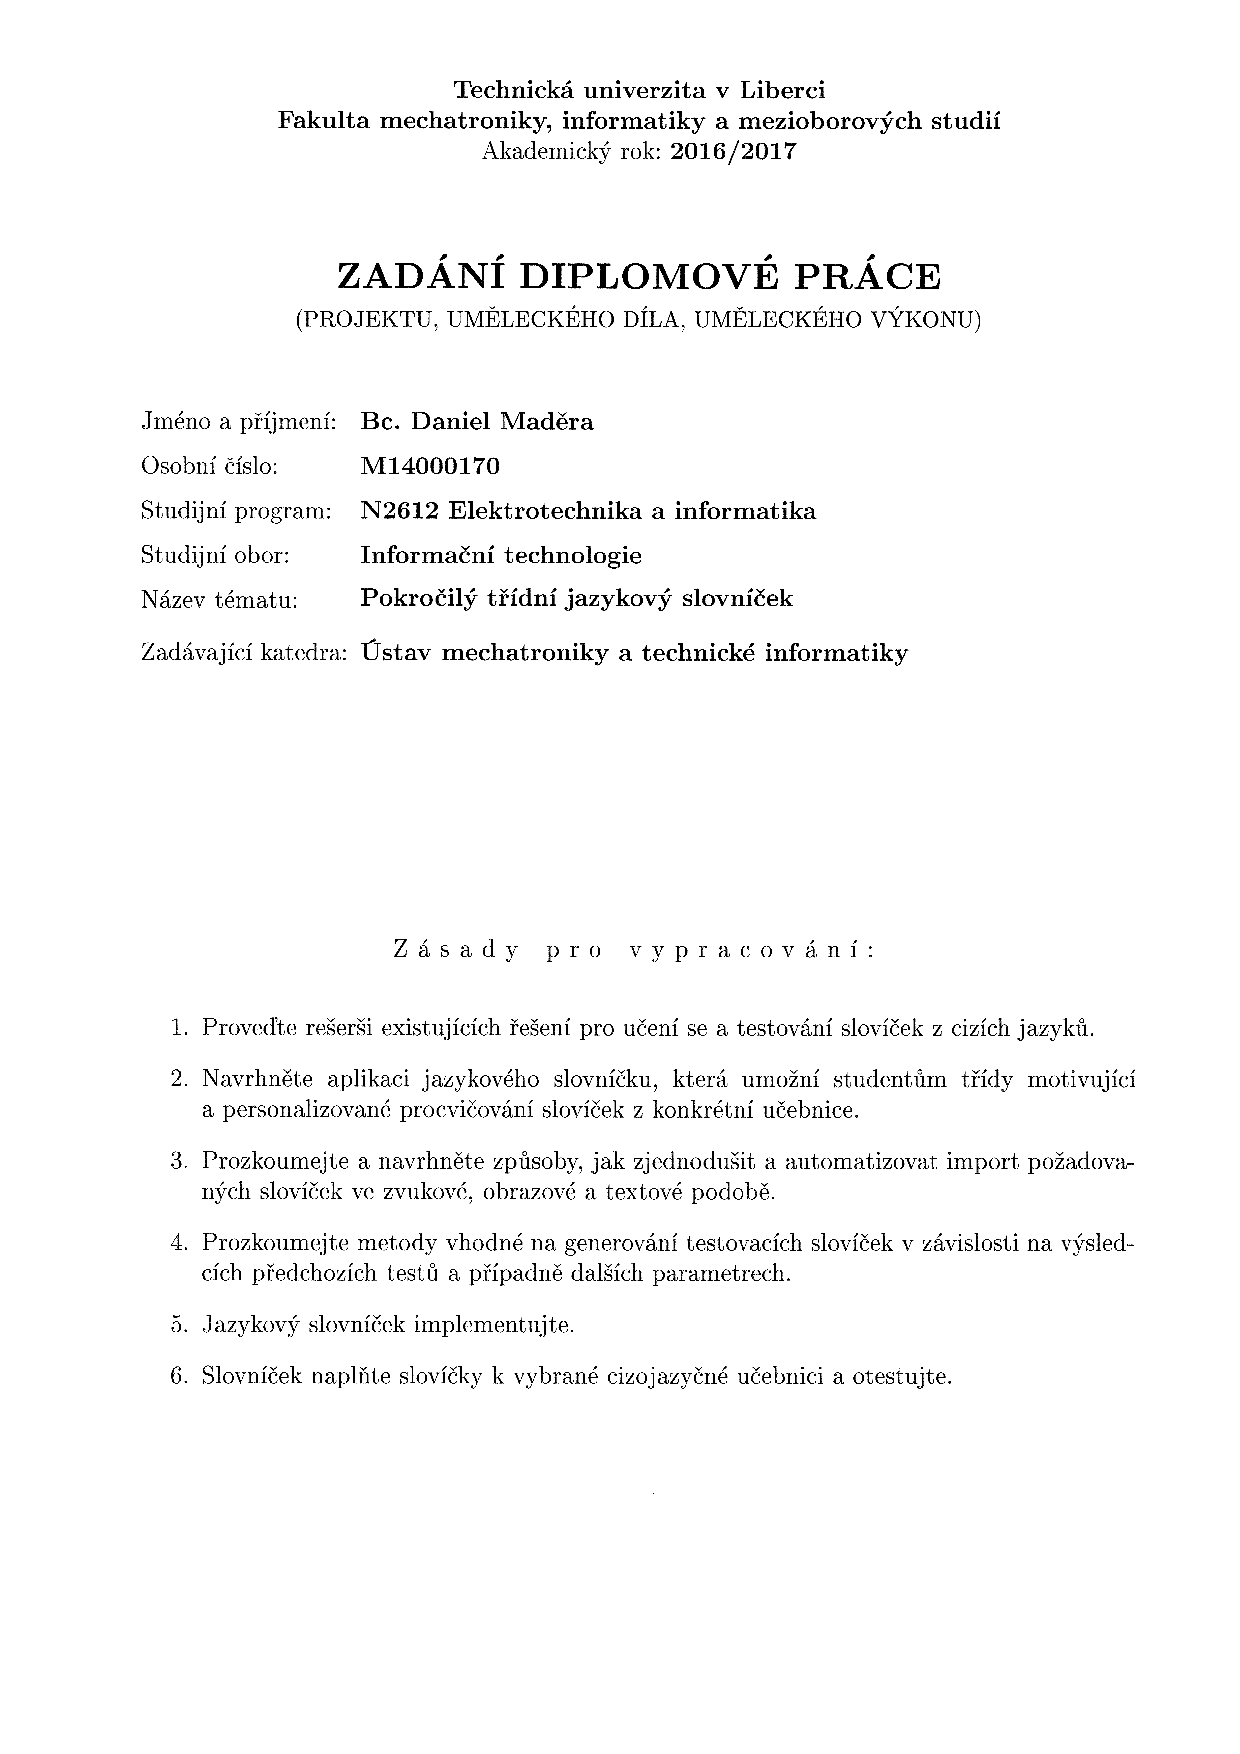
\includepdf[pages={1,2}]{zadani.pdf}
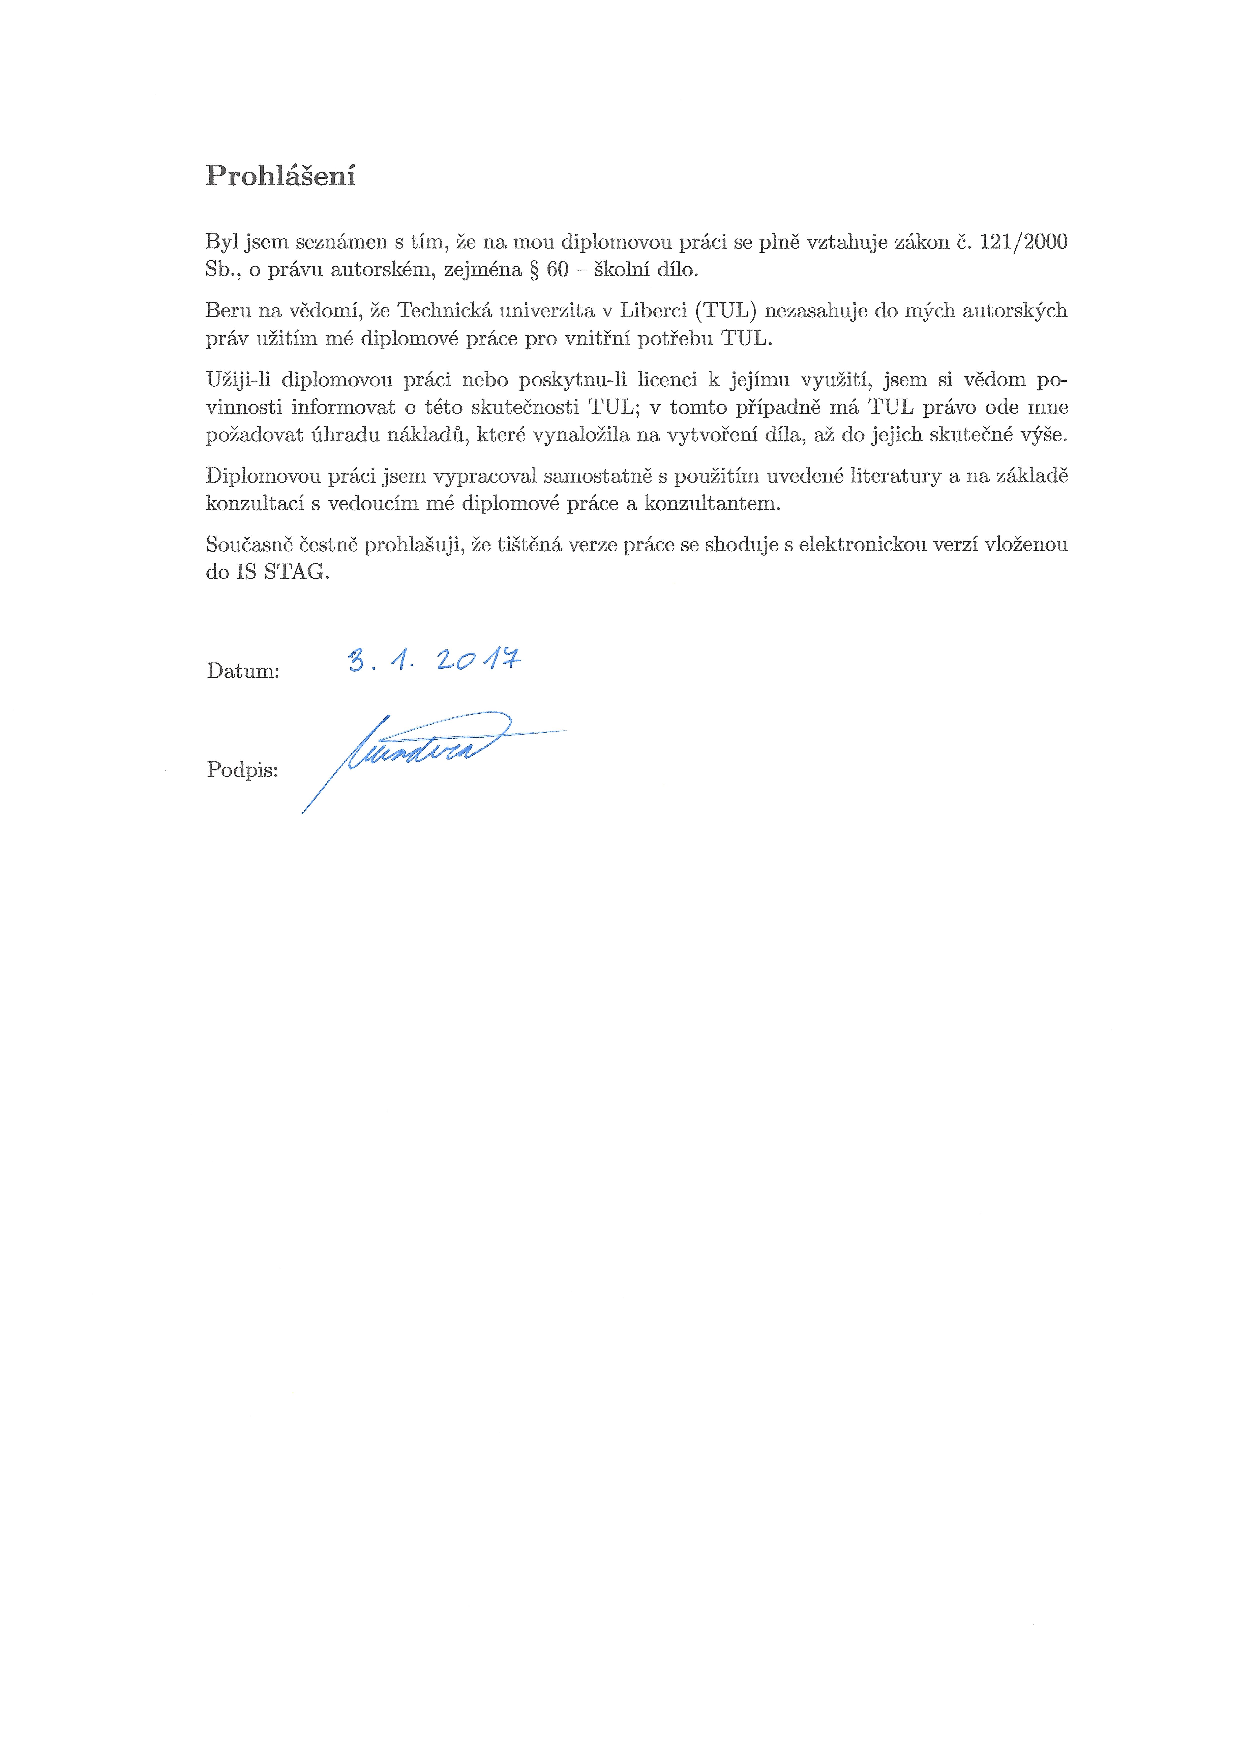
\includepdf{dp-prohlaseni-signed.pdf}
\setcounter{page}{5}

\newpage
\thispagestyle{plain}
\section*{Poděkování}
Rád bych touto cestou vyjádřil poděkování za trpělivost, užitečné rady a vedení práce Ing.~Janě Vitvarové, Ph.D. Rovněž bych rád poděkoval rodičům za podporu při psaní této práce a za umožnění studia.
\thispagestyle{empty}

\newpage
\thispagestyle{plain}
\section*{Abstrakt}
Tato práce se zabývá problematikou učení slovní zásoby cizího jazyka. Práce analyzuje a implementuje metody procvičování a připomínání slovíček za použití algoritmů rozloženého opakování. V rámci práce byla vytvořena aplikace v podobě webové služby jako učební nástroj, který má za úkol pomoci žákům s procvičením slov a rovněž k jejich permanentnímu zapamatování. Aplikace je složena z JavaScriptové SPA s podporou knihovny React a webového API v jazyce Python za použití Django frameworku. 

\section*{Klíčová slova}
učení slovíček, rozložené opakování, webové API, SPA, React, Django

\section*{Abstract}
This thesis deals with the issues of learning foreign language vocabulary. The thesis analyzes and implements methods of practicing and recalling vocabulary using spaced repetition algorithms. The thesis also describes a development of a web application as an educational tool that helps students practice foreign vocabulary. The application is designed to permanently improve recall of the vocabulary. The application is composed of a SPA written in JavaScript supported by the React library and a web API in Python using the Django framework. 

\section*{Keywords}
vocabulary learning, spaced repetition, web API, SPA, React, Django

\thispagestyle{empty}

\newpage
\thispagestyle{empty}
\setcounter{tocdepth}{2}
\tableofcontents


\newpage
\thispagestyle{empty}
\listoffigures
\listoftables
\renewcommand{\lstlistingname}{Ukázka kódu}
\renewcommand{\lstlistlistingname}{Seznam ukázek zdrojových kódů}
\lstlistoflistings

\newpage
\thispagestyle{empty}
\printglossary[title=Seznam zkratek]
\cleardoublepage

\section{Úvod}
    % proč se zaobývat tímto tématem
    Výuka cizích jazyků je pro aktuální společnost jedna z nejzásadnějších otázek, ať se jedná o pracovní příležitosti v zahraničí nebo o sociální problematiku světa. Žáci a studenti se často účastní různých kurzů nebo později studenti využívají Erasmus programů, kde převážně vyhledávají zlepšení komunikace v cizím jazyce. A právě slovní zásoba je pro rozvoj znalosti cizího jazyka ta nejzásadnější.

    Žáci si při výuce cizího jazyka obvykle vedou vlastní slovníček, do kterého zapisují nově nabytá slova. Problémem je, že slovíčka pouze zapíšou, a tím to končí. V době přípravy na test rychle slova zopakují a následně z krátkodobé paměti test napíšou, což má za následek, že pokud naučená slova dále neopakují, dojde k jejich zapomenutí. 

    Existuje řada řešení, které pomáhají rozvíjet vědomosti cizího jazyka. Problémem ale je, že tyto řešení pro žáky neposkytují přizpůsobení úrovně ani informací. Žáci jsou tudíž nuceni se učit jinou slovní zásobu než je ta, kterou aktuálně procházejí ve škole. Pro žáka je toto neefektivní a nevýhodné.

    Z výše uvedených důvodů vznikl námět na tuto práci. Cílem diplomové práce je provést analýzu, jak zefektivnit učení a motivovat žáky k procvičování slovíček. Na základě zjištěných poznatků navrhnout a implementovat aplikaci, která umožní rozvíjet cizojazyčnou slovní zásobu. A vyučujícím poskytne nástroj pro správu a prezentaci slovíček pro žáky. 

    Úvodem se práce zabývá rešerší existujících řešení podobných aplikací. Analýza rovněž zahrnuje shrnutí informací o rozvoji slovní zásoby cizího jazyka v podobě dostupných metod a technik k motivaci učení a k efektivnímu zapamatování slov. Na základě zjištěných informací z rešerše byla provedena specifikace požadavků, které sloužily jako hlavní podklad pro návrh aplikace popsaný v kapitole 2. V této kapitole jsou rovněž detailněji popsány způsoby generování testovací sady, průběh importu slov a vybrané metody zajišťující motivaci žáků. V kapitole 3 a 4 se práce zabývá implementací navržené slovníkové aplikace v podobě webové služby. Kapitola 3 se věnuje klientské části a kapitola 4 té serverové. V obou jsou představeny technologie, které jsou využívány pro vývoj, jejich implementace a průběh testování. 

    % neopakovat abstrakt, lehce nastínit zadání, jaká je motivace
    % popsat, jak je práce strukturovaná - rozcestník


\newpage
\section{Analýza}
    
    \subsection{Hlavní cíle}
        % jak si aplikaci představuji
        % zlepšení přípravy na hodiny cizího jazyka
        % shrnout v odstavci požadavky na aplikaci
        
        Hlavním cílem aplikace je připravit žáky na hodinu cizího jazyka a zároveň přirozeně rozvíjet slovní zásobu tak, aby studenti neztratili motivaci a chuť k poznávání nových výrazů. Dále také umožnit žákům se otestovat a ověřit, zda naučenou sadu slov ovládají. Aplikace by se měla adaptovat na zdatnost a úroveň každého ze žáků. Vyučujícím by aplikace měla usnadnit správu a import slovíček, která třída má umět v rámci dané učebnice a následně předkládat žákům vhodnou slovní zásobu, například jako přípravu pro následující lekci ve škole.

        \subsubsection{Personalizace}
            % personalizace podle potřeby konkrétní třídy - konrétní učebnice
            % personalizace podle potřeby jednotlivých žáků - generování na základě předcházejících výsledků
            Důležitým cílem aplikace by měla být adaptace (personalizace) aplikace podle potřeb jednotlivých žáků a celých tříd. Adaptace na úrovni žáka znamená, přistupovat k němu individuálně na základě jeho úrovně, znalostí a dovedností. V případě konkrétní třídy jde o individuální přístup, a to zejména v sadě slov, které je třeba v přípravě procvičovat. 

        \subsubsection{Motivace}
            Důležitou součástí obecného vzdělávání je motivace. To znamená přimět žáky, aby z vlastní iniciativy chtěli rozvíjet své vědomosti. Problém ale je, že se děti přirozeně neučí z vlastní vůle, ale aby uspokojili okolí. Motivace se rozdělují do skupin - vnitřní a vnější nebo pozitivní a negativní \cite{bib:motivace}. Analýza bude zaměřena pouze na motivační prostředky, které lze zařadit do aplikace na procvičování slovíček.

            Motivace založená na základě vlastních úspěchů je důležitá pro utvrzení sebevědomí žáků. Ocenění v případě zvládnutí sady slov nebo gramatického bloku lze v případě aplikace implementovat například hláškami s projevem pochvaly nebo jiným upozorněním na dosažený výsledek. Zajímavým prvkem v aplikaci by mohlo být i herní prostředí. Žáci si rádi hrají a již J. A. Komenský poukázal na důležitost her ve vzdělávacím procesu.

            % motivace dětí k učení slov (vrámci třídy)
            % motivace - přispění k úspěchu třídy
            % motivace - vlastní úspěchy

            Jedním z dalších stěžejních faktorů motivace je kolektiv. Právě díky kolektivu, ve kterém funguje přirozená rivalita, jsou žáci schopni dosáhnout mnohem vyšších výsledků, než kdyby se vzdělávali odděleně a samostatně. Rivalita a soutěživost se může projevovat i velmi negativním způsobem. Místo kamarádských vztahů mezi dětmi mohou vznikat nepřátelské vazby, ve kterých dochází k posměchu méně nadaných dětí, a ty se potom necítí v kolektivu dobře. Zajímavější motivací pro kolektiv je například vidina společně dosažených výsledků. V případě učení slovíček by to byl počet slovíček naučených za rok v rámci celé třídy. Dochází zde k utužování kolektivu a děti by mohlo těšit to, že nějakým způsobem přispívají k úspěchům celé třídy.

        \subsubsection{Využití IT pro výuku}
            Posledních několik let se společnost ubírá trendem informačních technologií. Každý ze žáků má už od útlého věku přístup k počítači nebo k chytrému telefonu. Orientace a schopnost tato zařízení používat není pro děti žádný problém. Přirozeně se tedy tato zařízení postupně stávají součástí každodenní přípravy žáka na následující školní den. V některých případech plně nahrazují klasické učebnice a jsou přímo začleněny do výuky. Použití informačních technologií má za následek i zlepšení motivace při výuce. Obecně je známo, že žáci raději studují slovíčka interaktivní formou hádanek, křížovek nebo her, než nekonečných seznamů slov.

            Důležitost cizích jazyků se projevuje na míře používání například chytrých tabulí nebo tabletů při výuce. Tato zařízení umožňují interaktivní výuku, kde lze využít nejen textových, ale také obrázkových a zvukových prostředků pro lepší zasazení nově nabytých vědomostí do kontextu. 

            % výuka cizích jazyků - smartboards            
            % vysoká motivace dětí pracovat s PC

    \subsection{Existující řešení}
        Na trhu lze nalézt nepřeberné množství aplikací pro výuku cizích jazyků. Řada z nich jsou téměř komplexní systémy, které provází studenta od základních frází a slovíček až po gramatické standardy cizího jazyka. Analýza existujících řešení byla zaměřena na aplikace, které se zabývají především testováním slovíček a frází.

        Do analýzy existujících řešení byly zahrnuty tři desktopové, jedna webová a jedna mobilní aplikace.

        \subsubsection{TS Angličtina}
            Z analyzovaných řešení se jevila desktopová aplikace TS Angličtina od firmy Terasoft ta nejlépe funkčně propracovaná. Tato firma se zabývá širokou škálou výukových nástrojů se zaměřením na základní školy. V případě cizích jazyků se zabývají výukou anglického a německého jazyka. Hlavní předností aplikace je podpora nejvíce používaných učebnic cizího jazyka. Aplikace umožňuje testování různými způsoby - psaný překlad slova, porozumění mluvenému slovu, vybírání správných významů nebo doplňování vynechaných slov \cite{bib:terasoft}. Analýza byla tvořena pouze z webových informací o produktu od vydavatele. Bohužel firma Terasoft neposkytuje DEMO nebo TRIAL verzi aplikace, která by hlubší analýzu umožňovala.

        \subsubsection{Langsoft Teacher}
            Dalším analyzovaným řešením byla aplikace Langsoft Teacher, která je dostupná nejen v podání desktopové aplikace, ale také i mobilní aplikace pro platformy iOS a Android. Aplikace je velmi komplexní, obsahuje různé moduly pro testování například v obrazové formě pro předškolní děti. Zajímavá vlastnost, kterou aplikace disponuje, je pamatování problematických slov a nabízení těchto slov častěji než těch bezproblémových. Dále program umožňuje automaticky rozšiřovat slovní zásobu, která je v testování zahrnuta \cite{bib:langsoft}.

        \subsubsection{Duolingo}
            Dalším v pořadí byla aplikace Duolingo. Jedná se o mobilní aplikaci pro Android. Zahrnuje učivo cizího jazyka od základních komunikačních frází až po tvorbu gramaticky složitějších vět. V aplikaci je připravena dlouhá řada cizích jazyků - němčina, angličtina, španělština, italština a další. Chybí ale více referenčních jazyků. Aktuálně lze využít pouze angličtinu. Aplikace kromě standardních funkcí zahrnuje i rozpoznávání mluvených odpovědí. Zajímavým poznatkem byl systém motivace uživatelů, kde si každý mohl pozvat své přátele, mezi kterými docházelo k sdílení dosažených výsledků. Dalším motivačním základem bylo nutkání udržení plánu pravidelného testování, jelikož v opačném případě docházelo k automatickému zvyšování objemu testovacích dat. Nevýhodou aplikace byla nutnost připojení k internetu. V případě požití mobilních dat, docházelo ke zpoždění zejména při rozpoznání slov.

        \subsubsection{Vocabulary Trainer}
            Vocabulary Trainer je webová aplikace zdarma, napsaná v jazyce PHP, která naučí 5000 nejvíce používaných slov daného jazyka. Aplikace umožňuje hodně možného nastavení. K dispozici je i řada jazyků včetně češtiny a to jako referenční i jako učený jazyk. Testování spočívá nejdříve ve čtení slov. A následně uživatel vybírá odpověď z daným možností. Aktuálně překládané slovo si lze kdykoliv přehrát v různé rychlosti. Jako motivační základ aplikace využívá jednoduchý bodový systém. Součástí je i kalendář s emailovou upomínkou k dalšímu testování. Program je propracovaný, ale poměrně pomalý a dlouho trvá zejména úvodní načítání dat. Její výrobce LanguageCourse S.L. poskytuje i mobilní aplikaci pro Android k učení anglických slov a frází.

        \subsubsection{Supermemo aplikace}
            \label{supermemo-app}
            Za zmínku ještě stojí aplikace Supermemo. Není to aplikace s připravenými daty k testování slov cizího jazyka, ale slouží čistě jako šablona pro testování jakéhokoliv druhu otázek. Aplikace implementuje algoritmus Supermemo, který je založen na metodě postupného zvyšování intervalu dotazování na naučené informace. Při každé odpovědi program spočítá, kdy by si uživatel měl danou otázku zopakovat tak, aby odpověď byla správná a zároveň se co nejvíce zvyšoval interval mezi aktuální a předchozí odpovědí. Aplikace se adaptuje na schopnosti uživatele, v přiměřeném měřítku buď zvyšuje nebo snižuje interval dalšího připomenutí.

        % možné ještě rozvést aplikaci EasyWords

        % žádná z aplikací neumožňuje personalizované učení 
        % ve škole (z učebnice) se učí jiná slovíčka než v aplikacích
        % po otestování slova nedochází k jeho znovu připomenutí

        Z výše uvedených aplikací až na Supermemo žádná neumožňuje personalizovaný výběr učiva. Tedy nelze vložit vlastní slovíčko nebo si určit sadu slov pro testování. Proto jsou tyto aplikace především cílené pro uživatele, kteří vnímají výuku jazyka jako samostatné vzdělávání sami sebe. Pro žáky, kteří absolvují lekce z cizího jazyka ve škole je tento typ vzdělávání nevyhovující, jelikož se musí učit dvě nezávislé skupiny slov. Sice dochází k rozvinutí slovní zásoby studenta i do jiných okruhů než je jeho učebnice. Ale málokterý student má ještě energii, časovou dotaci a vlastní iniciativu na to, aby se připravoval na školní test ze slovíček a ještě rozvíjel samostatně svoji cizojazyčnou slovní zásobu.

    \subsection{Učení slovíček}
        % problematika malých dětí a učení slov
        % Biemiller and Boote (2006)
        % ročně se dá zvládnout maximálně 400 slov u studentů 2 - 5 třídy
        % docházelo k zvýšení učenlivosti, když studenti si mohli zapsat 
        % slovo vlastní definicí
        Standardně učení slovní zásoby cizího jazyka je založeno na častém opakování slov. Dle výzkumu Biemillera a Boote se lze ročně zvládnout až 400 slov u studentů 3.—6. tříd \cite{bib:beimiller}. Což je v případě cizího jazyka poměrně velké číslo, ale problém je, do jaké míry je slovo správně ukotveno v dlouhodobé paměti. Porovnání, kolik je potřeba slov pro ovládnutí anglického jazyka, usnadní následující tabulka \ref{tab:english-vocab-usage}, která zahrnuje procentuální využití nejvíce používaných slov v každém z odvětví \cite{bib:learning-vocab}. 

        \begin{table}[ht!]
            \centering
            \begin{tabular}{|l|c|c|c|}
            \hline
            & \multicolumn{1}{l|}{Konverzace} & \multicolumn{1}{l|}{Noviny} & \multicolumn{1}{l|}{Akademický text} \\ \hline
            1. 1000 slov & 84,3\% & 75,6\% & 73,5\% \\ \hline
            2. 1000 slov & 6\% & 4,7\% & 4,6\% \\ \hline
            Akademické výrazy& 1,9\% & 3,9\% & 8,5\% \\ \hline
            Ostatní & 7,8\% & 15,7\% & 13,3\% \\ \hline
            \end{tabular}
            \caption{Používání slov v britské angličtině}
            \label{tab:english-vocab-usage}
        \end{table}

        \subsubsection{Zastaralý způsob učení}
            Dle vlastního průzkumu žáci základních škol nevyužívají k učení slovíček nikterak pokročilé technologie. Většinou si udržují vlastní slovníček, do kterého si poznamenávají nově nabytá slova. Při učení zakrývají část s cizojazyčnými slovy a na základě českého ekvivalentu se snaží vybavit překlad slova. Tato metoda neposkytuje prakticky žádnou zpětnou vazbu. Žáci většinou pouze do krátkodobé paměti uloží slova, později při testu rychle zodpoví a následně během pár hodin si na slovo už ani nevzpomenou. Nevýhod má tato metoda celou řadu, ale jednou z klíčových vad je, že si žáci nevytvoří dostatečně souvislostí, aby řádně ukotvily slovo v paměti.

        \subsubsection{Zvuková interpretace}
            Zejména v učení cizího jazyka je zvuková podoba a interpretace slov velice důležitá. Žák díky znění slova získá podvědomí o dialektu daného jazyka a zároveň dochází k lepšímu zapamatování slova. Právě díky zvukům dochází k propojení při učení i pravé mozkové hemisféry, což napomáhá k vytvoření pevnějšího ukotvení v paměti. Dle studie bulharského vědce George Lozanova, který se zabýval studiem mozku a učebních metod, byl zjištěn obrovský přínos zvukových vjemů \cite{bib:suggestology}.

        \subsubsection{Problematika obtížnosti}
            % každý z žáků má indiviální úroveň znalostí cizího jazyka
            % a každý z žádů se jiným tempem učí cizojazyčná slovíčka
            Velkým problémem v učení slov je přizpůsobit obtížnost každému ze žáků individuálně. Jelikož ne všichni mají stejnou úroveň znalostí cizího jazyka a každý potřebuje jiné tempo pro zapamatování sady slov. Jsou žáci s výbornou pamětí, kterým stačí si slova pouze jednou přečíst a dokáží je používat. Ale jsou i žáci, kterým nestačí je pětkrát zopakovat. Dalším problémem je obtížnost z pohledu jednotlivých slov. Každé slovo má odlišnou obtížnost, kterou lze soudit například podle míry používanosti v jazyce, délky slova, zdali obsahuje přehlasování, dvojitá písmena nebo podobnost s referenčním slovem.

        \subsubsection{Učení slov v kontextu}
            % jak je důlžité se slova učit v kontextu - použití ve větě z učebnice
            % drive/vocab-techniques.pdf
            Pro učení slov cizího jazyka je rovněž důležité správné zasazení významu slova do kontextu. Dle průzkumu Biemillera a Bootea z roku 2006 bylo zjištěno, že u žáků od 10—13 let docházelo k nárůstu zapamatovaných slov o 4\%, pokud byla slova předložena v kontextu vět. Důležitým poznatkem z tohoto průzkumu je, že žáci si nejen déle naučené slovo pamatovali, ale správně ho i interpretovali, když ho měli za úkol svými slovy vysvětlit \cite{bib:beimiller}. Ve stejném průzkumu rovněž docházelo ještě k vyššímu zlepšení v učení, kdy si žáci zapisovali vlastními slovy definici a použití slova.
        
    \subsection{Testování slovíček}
        % drive/accesing-vocabulary-in-the-language-classroom.pdf
        % důležitost aktivní slovní zásoby pro výuku cizího jazyka

        \subsubsection{Aktivní a pasivní slovní zásoba}
            % co je aktivní a pasivní
            Slovní zásobu, kterou využíváme k tvorbě vět, ať už v cizím nebo mateřském jazyce, rozdělujeme na dvě skupiny - aktivní a pasivní. Pasivní zásoba je sada slov, která jsou pevně a spolehlivě uložena v naší paměti. Průměrný žák zná cca 50 000 výrazů. Velikost pasivní zásoby je ovlivněna věkem, vzděláním a četbou. Slova ze této sady využíváme zejména při písemné formě, ať už se jedná o čtení nebo psaní. Aktivní zásoba je sada slov, ve které lze najít žádané slovo během desítek milisekund. U většiny lidí dosahuje velikosti 4 000 až 8 000 výrazů \cite{bib:lexikologie}. Slovo se díky používání dostává z pasivní do aktivní slovní zásoby. 

        \subsubsection{Metody testování}
            \label{test-methods}
            % pasivní vs aktivní
            % aktivní - vzpomenutí, rozpoznání

            Metod testování slovní zásoby je mnoho. Základní rozdělení je na pasivní a aktivní metody. V případě pasivních metod se jedná například o výběr z nabídnutých možností. Jde o případ, kdy student nemusí znát přesnou odpověď, ale dokáže otázku vyhodnotit správně vylučovací metodou. Při aktivním testování žáci musí odpověď znát, aby otázka byla vyhodnocena správně. Pasivní metoda má pozitivní vliv například na motivaci žáka, který u ní tolik netápe a za pomoci zdravého rozumu může test vyhodnotit správně. Problém ale vzniká při používání získaných a procvičených informací. V případě cizího jazyka lze pasivní slovní zásobu využít pro čtení a náslech, ale pro ovládnutí cizího jazyka je nedostatečná a tudíž nevhodná. 

            Dalším rozdělením pasivního a aktivního testování slovíček je rozpoznávání (\textit{recognition}) a vzpomenutí (\textit{recall}). Rozpoznávání spočívá v předložení cizího slova žákovi, který pro správné zodpovězení musí najít český ekvivalent. Vzpomenutí je způsob testování opačným způsobem než rozpoznání. Uživateli je předložen výraz v jeho mateřském jazyce a on musí nalézt správný výraz v cizím. Rozpoznání je z principu jednodušší pro uživatele než vzpomenutí. Lze ho tedy využít rovněž pro zvýšení motivace při procvičování slov. Ale pro ověření, zda je slovo ovládnuté či nikoliv je metoda rozpoznání také nedostatečná.

        \subsection{Typy testů}
            % multiplechoice, matching, completion, translation
            % vyžití her - problém je, že tento způsob většinou není ani efektivní, jelikož si procvičí například v případě doplňování písmen pouze pár slov za poměrně dlouhý čas

            V analýze existujících řešení bylo procvičování a testování slov interpretováno různými způsoby. Obecně by se typ testů dal rozdělit na tři kategorie - textové testy, multimediální a herní testy.

            \subsubsection{Textové testy}
                Textové testy se vyskytovaly například jako výběr z více možností nebo spojováním spolu souvisejících významů, jak už ale bylo uvedeno v kapitole \ref{test-methods}, jedná se o rozvíjení pasivní slovní zásoby. Zajímavějším typem testů je doplňování slov do vět a klasický překlad slova. Tyto typy rozvíjejí žádanou aktivní slovní zásobu. V existujících řešeních textové testy byly doplněny zvukovou interpretací cizího slova.

            \subsubsection{Multimediální a herní testy}
                Zajímavým využitím multimédií by mohlo být zahrnutí otestování výslovnosti. Tedy možnost nahrání odpovědi a následně by došlo k rozpoznání. Ale analýza a rozpoznání řeči není nikterak triviální záležitost. Dalším zajímavým řešením byly herní testy. Díky nim docházelo k zvýšení motivace uživatelů. Problém je, že tento typ procvičování většinou není zas tolik efektivní, jelikož si uživatel procvičí například v případě doplňování písmen do křížovky nebo známé hry \textit{Hangman} pouze pár slov za poměrně dlouhý čas.

        \subsection{Metoda rozloženého opakování}
            \label{spaced-repetition}
            % obecně o metodě 
            Až na výjimečné paměti je obecně známo, že pokud chceme informaci v paměti uchovat dlouhodobě, je nutné ji opakovaně připomínat. Pokud informace není vyžívána, s největší pravděpodobností dojde ke ztrátě této informace. V případě, že uživatel s touto informací pracuje častěji, výrazně navyšuje šance pro její zapamatování. Metoda rozloženého opakování (\textit{spaced repetition}) je učební technika založená na opakovaném připomínání informace se zvyšujícím se intervalem\cite{bib:spaced-rep}. Na začátku učebního procesu, jsou intervaly krátké například na hodinu, 4 hodiny nebo celý den. S postupem se tyto intervaly mohou zvyšovat až na týdny a měsíce. Ideální systém rozloženého opakování nabídne zopakování informace těsně před tím, než dojde k jejímu eventuálnímu nevzpomenutí.

        \subsubsection{Křivka zapomínání}
            Křivka zapomínání je graf exponenciálního charakteru, který znázorňuje, za jak dlouho a s jakou pravděpodobností je možné si na nově nabytou informaci vzpomenout. První tuto křivku specifikoval už v roce 1885 Hermann Ebbinghaus. Na ose Y lze nalézt procentuální pravděpodobnost vzpomenutí na informaci, na ose X je čas. V čase 0 dojde k nabytí informace a s postupem času dochází k zapomínání. U průměrných pamětí dojde k potencionálnímu zapomenutí nové nesouvisející informace bez kontextu během pěti dní \cite{bib:ebbinghaus}.

            Následující obrázek \ref{fig:forgetting-curve} znázorňuje metodu rozloženého opakování na křivce zapomínání. V čase s 80\% pravděpodobností vzpomenutí na danou informaci dojde k připomenutí. Křivka zapomínání se posune na ose Y a znovu dochází k postupnému zapomínání. Díky exponenciálnímu charakteru interval mezi jednotlivými opakováními narůstá také exponenciálně. V ideálním případě se posune exponenciála tak, že se bude limitně blížit 80\% hranici.

            \begin{figure}[ht!]
                \centering
                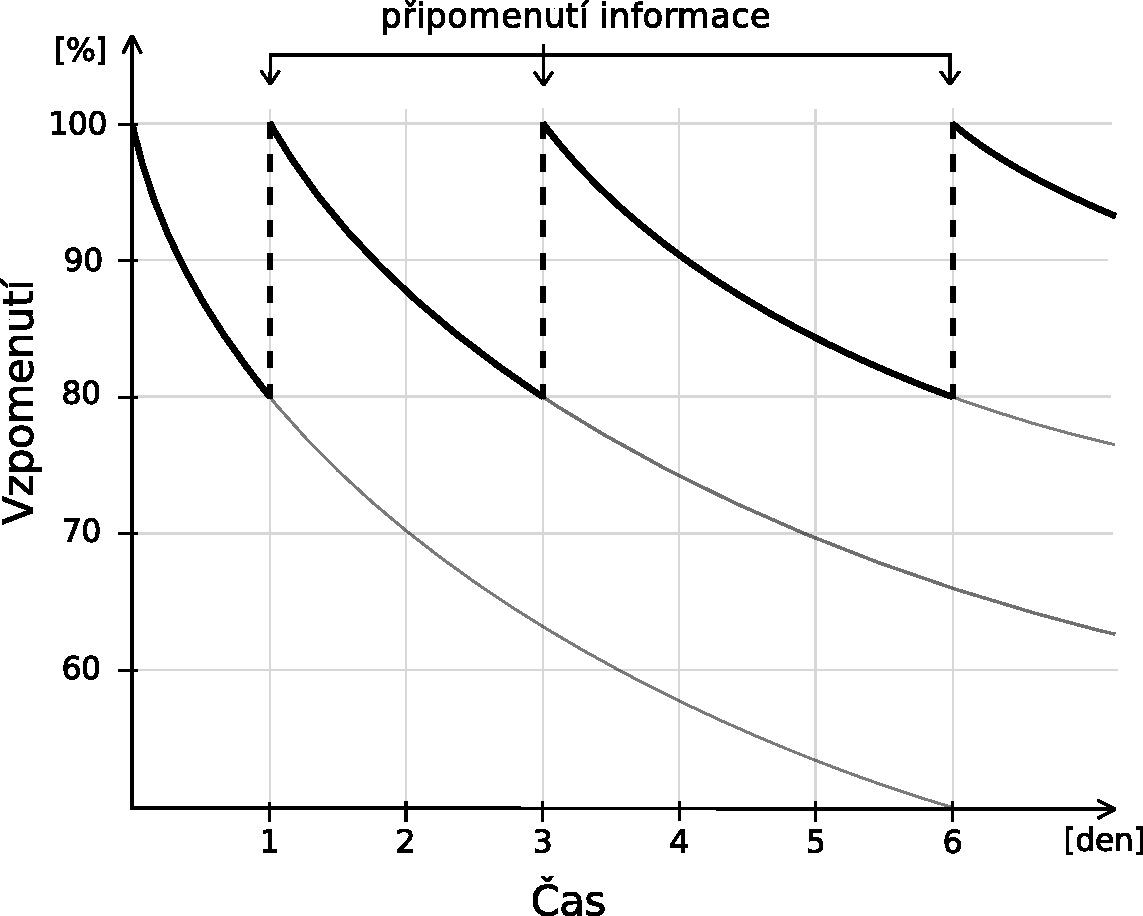
\includegraphics[scale=0.55]{../diagrams/forgetting-curve.pdf}
                \caption{Naznačení rozloženého opakování na základě křivky zapomínání}
                \label{fig:forgetting-curve}
            \end{figure}
         
        \subsubsection{Leitnerův algoritmus}
            % shrnout leitnerův algoritmus
            \label{leitner}
            Na Leitnerův algoritmus lze nahlížet jako na známý učební postup v podobě karet s otázkami. Tyto karty jsou rozděleny do skupin, které jsou označeny například 1 až 3. Kategorií ale obecně může být více. Nová karta je zařazena do první kategorie. Karty v první kategorii jsou opakovány častěji. V poslední kategorii jsou karty opakovány méně častěji. Karty jsou přemisťovány podle toho, jak uživatel zvládá odpovídat na jednotlivé otázky. V případě, že uživateli otázka na kartě nedělá problémy, přesune kartu do vyšší kategorie. V opačném případě, kdy si uživatel nemůže vzpomenout na danou otázku, karta se přesune do první kategorie a cyklus pro danou kartu začíná znovu.

    \subsection{Specifikace požadavků}
        % číselný seznam toho, co má aplikace dělat
        Na základě analýzy byla provedena specifikace požadavků, které budou implementovány v aplikaci pro testování slovíček z cizího jazyka.

        \begin{enumerate}
            \item správa učebnic
                \begin{itemize}
                    \item tvořit, editovat a mazat vlastní učebnice
                \end{itemize} 
            \item správa slovíček v učebnici
                \begin{itemize}
                    \item tvořit, editovat a mazat slovíčka
                    \item hromadně slovíčka do učebnice importovat
                    \item částečně automatizovat zvukovou a obrazovou interpretaci slovíčka
                \end{itemize} 
            \item správa modulů a tématických okruhů v učebnici
                \begin{itemize}
                    \item tvořit, editovat a mazat moduly učebnice
                    \item přiřazovat slovíčka do daných modulů
                \end{itemize}
            \item správa uživatelských skupin (tříd)
                \begin{itemize}
                    \item tvořit, editovat a mazat uživatelské skupiny
                    \item umožnit uživatelům se přihlásit do skupiny
                \end{itemize}
            \item správa testovacích sad
                \begin{itemize}
                    \item tvořit, editovat a mazat testovací sady
                    \item umožnit vybírat slova pro testovací sadu z vlastních i veřejných učebnic
                    \item přiřazovat testovací sady ke skupinám uživatelů
                \end{itemize}
            \item procvičování slovíček
                \begin{itemize}
                    \item vybrat testovací sadu slovíček
                    \item generovat slova na základě úrovně uživatele
                    \item zahrnout obrazovou a zvukovou interpretaci do procvičování
                    \item možnost uložit stav testování a umožnit pozdější navázání
                \end{itemize}
            \item připomínat a procvičovat ovládnutou slovní zásobu 
            \item motivace
                \begin{itemize}
                    \item motivovat v rámci uživatelské skupiny
                    \item motivovat vlastní iniciativu k procvičování
                \end{itemize}
        \end{enumerate}


\newpage
\section{Návrh aplikace}
    % usecase diagram
    % jednotlivé use-case by měly být názvy jednotlivých podkapitol v návrhu aplikace
    Na základě specifikace požadavků byl vytvořen USE-CASE diagram aplikace. Diagram na obrázku \ref{fig:use-case} znázorňuje pouze obecné bloky funkčnosti aplikace. V následujících kapitolách bude každý z jednotlivých USE-CASE bloků popsán detailněji.

        \begin{figure}[ht!]
            \centering
            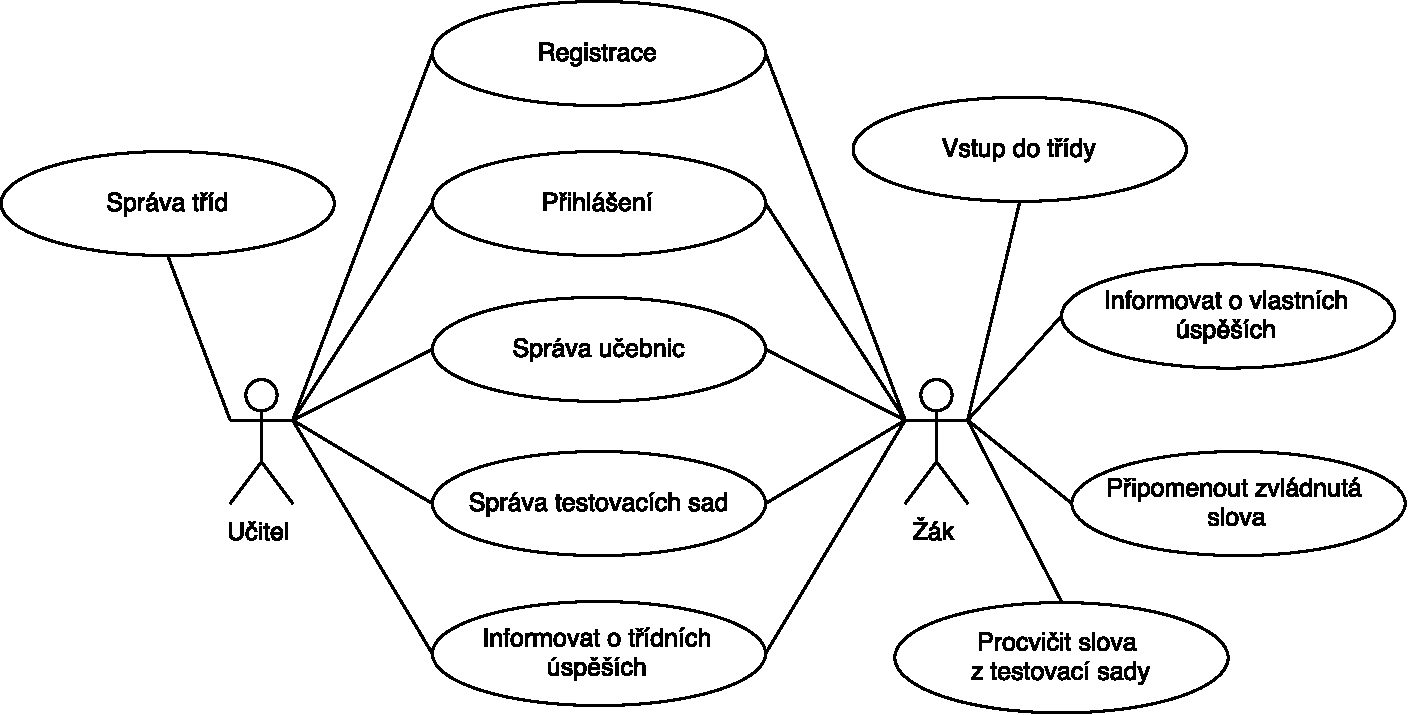
\includegraphics[scale=0.63]{../diagrams/use-case.pdf}
            \caption{USE-CASE diagram aplikace}
            \label{fig:use-case}
        \end{figure}

    \subsection{Uživatelské role}
        % rozvést rozdíl mezi žákem a učitelem - rovnocenné partnerství, každý může být učitel a student
        Do aplikace by měly vstupovat dva typy uživatelů - učitel a žák. Učitel z principu má za úkol spravovat testovací sady, učebnice a třídy. Žáci oproti nim mají za úkol vstupovat do svých tříd, procvičovat slova z testovacích dat, které jsou připravené od učitele a připomínat si zvládnutá slova. 

        Po konzultacích s vedoucím práce a vyučujícím cizího jazyka na základní škole došlo k několika změnám v návrhu právě v oblasti uživatelských rolí a i v principu aplikace. Vznikl požadavek, že aplikace by mohla fungovat spíše jako portál pro vzdělávání a ne jako výukový nástroj pro učitele. V návrhu tudíž vzniklo rovnocenné partnerství mezi učitelem a žákem.

        \subsubsection{Sjednocení uživatelských skupin}
            Podnětem pro sjednocení uživatelských skupin bylo umožnit žákům procvičovat si slova i v případě, že nejsou součástí žádné třídy. Tak aby se mohl kdokoliv do aplikace přihlásit, vybrat si testovací sadu a vyzkoušet svoje znalosti slovíček. Tato funkce umožňuje žákům volnější přístup k výuce. Nebylo totiž v požadavcích, aby měl učitel přehled o znalostech žáka - právě naopak. Účelem aplikace je poskytnout žákům možnost se samostatně vzdělávat a procvičovat slovní zásobu, a ne vyučujícím poskytnout nástroj pro otestování, zda žák disponuje požadovanými znalostmi. 

    \subsection{Správa učebnic}
        % sdílení učebnic (otevřený systém)
        % přijít do aplikace a jen tak si protestovat slova z učebnice
        % nemusí být člověk součástí žádné skupiny
        Z důvodu personalizace slovíček bylo nutné v návrhu aplikace zařadit učebnice, díky nimž si žáci budou procvičovat pouze slovíčka, která jsou pro ně aktuální ve výuce cizího jazyka. Učebnice obsahují moduly a v modulech se nacházejí jednotlivá slova. Při tvorbě učebnice bude zvolen cizí jazyk, pro který je učebnice připravená. V rámci jedné učebnice jsou slova unikátní. Tzn. do konkrétní učebnice nemohou patřit dvě stejná slova. Majitel učebnice je může editovat, vytvářet a mazat i v případě, že je využívána některým z ostatních uživatelů. 

        V aplikaci se může vyskytovat i více stejných učebnic. Například dva různí vyučující vedou své hodiny cizího jazyka podle stejné učebnice, ale každý si chce přizpůsobit sadu slov po svém. Proto se v aplikaci musí učebnice identifikovat majitelem a názvem učebnice.

        \subsubsection{Sdílení učebnic}
            Jelikož aplikace slouží jako portál pro vzdělávání, ve výchozím stavu jsou učebnice a slovíčka v nich veřejně přístupná jakémukoliv uživateli. Příchozí uživatel si tedy bude moci buď vytvořit vlastní učebnici se svými slovy, které si chce procvičit, nebo si může vybrat slova už z vytvořených učebnic. Díky sdílení si nový uživatel může prakticky okamžitě po přihlášení začít procvičovat slova bez nutnosti tvorby učebnice. Tento přístup je cílený právě především pro žáky, kteří si chtějí samostatně procvičovat slova a nepatřit do žádné konkrétní třídy.

        \subsubsection{Import slov do učebnice}
            Pro usnadnění zadávání dat je v aplikaci umožněno importovat celou sadu slovíček z učebnice. Původní myšlenkou bylo vytvořit parser, který bude schopný přečíst slovíčka přímo z učebnice ve PDF formátu. Po konzultaci s vyučujícím bylo rozhodnuto, že postačí import v podobě textového formátu odděleného čárkou. Důvodem je, že vyučující potřebují slovíčka postupně upravovat a doplňovat. Proto je pro ně sada slovíček v učebnici nevyhovující a spravují si vlastní slovníček a to nejčastěji ve formátu XLS aplikace Microsoft Excel. Z této aplikace není problém vyexportovat slova do textového formátu, kde hodnoty jsou oddělené čárkou.

    \subsection{Správa slovíček}
        % výhody více forem - lepší zapamatovatelnost
        % vytvoření hlubších asociací

        Jednotlivá slovíčka se budou ukládat do modulů učebnice. Slovíčko se bude charakterizovat - překladem v cizím jazyce, významem v mateřském jazyce, definicí slova v cizím i mateřském jazyce a použitím ve větách z učebnice. Dalšími atributy, kterými slovíčko disponuje, jsou obtížnost a slovní druh. Slovíčko bude možné doplnit o multimediální interpretaci a to v podobě zvuku a obrázku.

        %% Možné rozšíření - přidat možnost více významů slova
        \subsubsection{Textová forma}
            % importováním sady slov (bez automatizace překladů)
            % editace definic a použití ve větách
            Textová forma slovíčka spočívá v překladu slova a jeho významu v mateřském jazyce. Pro zjištění významu slova se může využít již hotová aplikace. Například Google Translate poskytuje aplikační rozhraní pro překlady slov i celých vět. Jelikož se aplikace bude zabývat aktivním rozpoznáním a vzpomínáním, je vhodné neautomatizovat významy slov. Učebnice nebo učitelé se mohou s Google Translate lišit ve významech slov. Dalším problémem je cena využívání překladů z Google Translete, která je účtovaná měsíčně \$20 za 1 milion znaků \cite{bib:google-api}.

        \subsubsection{Zvuková forma}
            % z Google \gls{api} importovat zvukové nahrávky
            % shrnout omezení, problematiku
            % 60 minut měsíčně je zdarma
            Do aplikace by měla být implementována i zvuková interpretace slovíčka v cizím jazyce. Zvukové nahrávky mohou být zařazeny do aplikace dvěma způsoby - manuálně vlastními nahrávkami nebo využít Google Text to Speech \gls{api}, které Google poskytuje zdarma. Aplikace bude záznam lokálně ukládat, aby se co nejvíce omezilo využívání \gls{api}. Zvuková nahrávka bude získána při importu slovíček do učebnice. Zadávající uživatel si bude moci zvolit, k jakému slovu chce zvukovou interpretaci.

        \subsubsection{Obrazová forma}
            % vyhledání z Google Images \gls{api} na základě cizojazyčného slova
            % autor učebnice vybírá dané slovo z importovaných
            % omezení dotazů - neprovádí se plně automatiky
            Obrazová interpretace slovíčka bude rovněž získaná z Google Custom Search \gls{api}. Toto aplikační rozhraní není omezené a lze v parametrech omezit vyhledávání pouze na obrázky. Při importu si uživatel zvolí, pro jaká slovíčka chce obrazovou formu. Automatizace v tomto případě není vhodná, jelikož ne všechny slovíčka lze interpretovat jako obrázek. Uživatel si také bude moci zvolit obrázek z několika možností. Po vybrání obrázku bude vytvořena komprimovaná kopie souboru a uloží se rovněž zdroj, odkud je obrázek získán. Tato forma bude v aplikaci sloužit pouze jako nápověda pro žáky, díky níž si mohou ke slovíčku vytvořit hlubší asociaci. 

            % využití možnost hledání dle "Lze volně užívat nebo sdílet". Vytvoření kopie, 
            Díky Google Custom Search \gls{api} lze vyhledávání parametrizovat. Výrazem pro vyhledávání bude referenční slovo v cizím jazyce, jelikož cílový jazyk bude nejspíš anglický, německý nebo španělský, a všechny tyto jazyky jsou více rozšířené, než ten český. Dalším parametrem vyhledávání je omezení pouze na obrázky s licencí \uv{Volně užívat nebo sdílet}, která umožňuje obrázek zkopírovat a nekomerčně publikovat s uvedením zdroje. Google nezaručuje, pod jakou licencí se obrázek aktuálně na stránkách prezentuje. Proto je uživatel při výběru obrázku vyzván, aby zkontroloval licenci použití.

    \subsection{Obtížnost slovíček}
        % vygenerovaná obtížnost na základě délky slova, podobnosti s českým jazykem, přizpůsobena vyučujícím
        Při zadávání slova do učebnice bude automaticky vyhodnocena jeho obtížnost, která je rozdělena do čtyř kategorií - snadné, střední, těžké a nemožné. Vyhodnocení obtížnosti je založeno na kombinaci několika parametrů slova - jeho délky, podobnosti s českým ekvivalentem a dalšími atributy jako počet přehlasovaných písmen nebo počet výskytů dvojitých písem. V případě nevhodně vygenerované obtížnosti slova, uživatel ji bude moci opravit dle vlastního uvážení. Délka slova je prahově rozdělena do kategorií obtížnosti, následně bude vyhodnocena podobnost s významem pomocí Levensteinovy vzdálenosti popsané v podkapitole \ref{levenstein}. Poté následuje vyhodnocení přehlasování a dvojitých hlásek, které ale ovlivňují obtížnost už jen minimálně.

        \subsubsection{Výběr algoritmu}       
            Levenshteinova vzdálenost je velmi podobná známe Hammingově vzdálenosti s tím rozdílem, že Hammingova vzdálenost uvádí počet pozic se stejným symbolem v obou řetězcích. Kdežto Levenshteinova vzdálenost uvádí počet jednoznakových editací. Pro určení míry podobnosti mezi slovem v cizím jazyce a jeho překladem je vhodnější Levenshteinova vzdálenost, jelikož akceptuje řetězce s různou délkou a v případě, že písmeno chybí, je to vyhodnoceno pouze jako odstraněné písmeno a algoritmus pokračuje dál. V případě Hammingovy vzdálenosti vynechané písmeno naruší porovnávání zbytku řetězce.

        \subsubsection{Levenshteinova vzdálenost}
            \label{levenstein}
            Levenshteinova vzdálenost v informatice je míra rozdílu mezi dvěma řetězci. Pro výpočet vzdálenosti se využívá matice s rozměry velikostí délek řetězců. V podstatě je vzdálenost minimální počet jednoznakových úprav ve slově, aby vzniklo slovo referenční. Za jednoznakovou úpravu se považuje smazání, záměna nebo vložení písmene na dané místo\cite{bib:levensthtein}.

            Vzorec \ref{levenshtein} je matematický zápis Levenshteinovy vzdálenosti, kde $a$ a $b$ jsou řetězce $a(i)$ a $b(j)$ jsou indexované znaky v řetězcích. Výsledná vzdálenost je rovna hodnotě v matici $dist_{a,b}$ na pozici $dist_{a,b}(|a|,|b|)$, kde $|a|$ a $|b|$ jsou délky řetězců \cite{bib:levenshtein}.

            \begin{ceqn}
            \begin{align}
                \label{levenshtein}
                dist_{a,b}(i,j) = 
                \begin{cases} 
                    max(i,j) & min(i,j) = 0\\min
                        \begin{cases}
                            dist_{a,b}(i-1,j)+1\\dist_{a,b}(i,j-1)+1\\dist_{a,b}(i-1,j-1)+
                            \begin{cases}
                                0 & a(i) = b(j)\\1 & a(i) \neq b(j)
                            \end{cases} 
                        \end{cases} & min(i,j) \neq 0 
                \end{cases}
            \end{align}
            \end{ceqn}

            V případě, že se pohybujeme v matici v prvním sloupci a prvním řádku, přiřazujeme hodnoty 1 až délka řetězce $a$ do sloupce a 1 až délka řetězce $b$ do řádku. Tedy první sloupec a první řádek v matici slouží jako referenční inicializace. V generování matice se následně pokračuje a porovnávají se jednotlivé znaky. První položka v minimu je případ, kdy písmeno bylo odstraněno z $a$. Druhá položka je případ, kdy došlo k vložení znaku do $a$ na základě znaku v $b$ řetězci. A poslední položka je případ porovnání znaků. V okamžiku, kdy se znaky rovnají, hodnota vzdálenosti na diagonále zůstává. V opačném případě se přičítá jednička.

            Výpočet Levenshteinovy vzdálenosti dvou slov znázorňuje matice \ref{leven-matice}, kde dochází k porovnání českého slova \textit{cyklus} a anglického výrazu \textit{cycle}. Tučně je znázorněna cesta výpočtu. Prováděné jednoznakové operace jsou žádná, žádná, žádná, záměna, záměna a vložení.

            \begin{ceqn}
            \begin{align}
                \label{leven-matice}
                \begin{matrix}
                    &  & c & y & c & l & e \\
                    & \textbf{0} & 1 & 2  & 3 & 4  & 5 \\
                    c & 1 & \textbf{0} & 1 & 2 & 3 & 4 \\
                    y & 2 & 1 & \textbf{0} & 1 & 2 & 3 \\
                    k & 3 & 2 & 1 & \textbf{1} & 2 & 3 \\
                    l & 4 & 3 & 2 & 2 & \textbf{1} & 2 \\
                    u & 5 & 4 & 3 & 3 & 2 & \textbf{2} \\
                    s & 2 & 5 & 4 & 4 & 3 & \textbf{3} \\ 
                \end{matrix}
            \end{align}
            \end{ceqn}

        \subsubsection{Určení globální obtížnosti}
            % shrnutí o váženém průměru obtížnosti, jaké a v jaké váze faktory jako Levenshtein, přehlasování a dvojitá písmena tvoří určení obtížnosti slova
            Základním parametrem globální obtížnosti slova je jeho délka, která má váhu 4 v celkovém průměru jednotlivých hodnot obtížnosti. Na základě prahových hodnot je délka rozdělena do čtyř kategorií - $\langle1,6)$ je snadné, $\langle6,11)$ je střední a $\langle11,\infty)$ je slovo těžké. Dalším parametrem k určení obtížnosti je Levenshteinova vzdálenost mezi referenčním slovem a jeho překladem, jejíž váha je 2. Znovu zde figurují nastavitelné prahové hodnoty - v případě, že se procentuální podobnost (tj. $pp = (1-a/l)*100$; kde $l$ je délka slova a $a$ je počet jednoznakových editací) nachází v intervalu $\langle70,100\rangle$, je obtížnost nejlehčí; v intervalu $\langle30,70)$ je střední a v intervalu $\langle0,30)$ je slovo těžké. Přehlasování znaku a dvojitý výskyt stejného znaku mají oba stejnou váhu 1. Bez výskytu přehlasování a dvojitého znaku je obtížnost kvalifikována jako snadná, jeden výskyt je střední obtížnost a více výskytů je obtížnost vyhodnocena jako těžká.

    \subsection{Generování slov pro procvičování}
        % generování slov na základě motivace, obtížnosti 
        % základem je slova, která jsou problematická pro žáka generovat častěji než slova, 
        % která zvládá s přehledem
        % účel generování slov má procvičit slova tak, aby byly správně ukotveny v dlouhodobé paměti a ne pouze v té krátkodobé
        Způsob generování slov je důležitý pro správné ukotvení slova v dlouhodobé a ne krátkodobé paměti. Při testování bude docházet i k několikanásobnému opakování slova. Základem generování je častěji a vícekrát předkládat slova, která jsou pro žáka problematická a slova, která jsou zvládnuta žákem s přehledem, jsou méně častěji testována. Pro generování byla zvolena metoda rozloženého opakování v podobě přizpůsobeného Leitnerova algoritmu, který je popsán v kapitole \ref{leitner}.
        
        Algoritmus pro procvičování slov se dělí na dvě části. V první části se zjišťuje, jaká slova jsou pro zkoušeného uživatele jednoduchá a naopak s jakými slovy má problém - tato fáze se bude dále nazývat inicializační. Po této fázi následuje fáze s použitím Leitnerova algoritmu - tato fáze bude nazývána testovací.

        \subsubsection{Inicializační fáze}
            \label{init-faze}
            % setřídění slov nejlehčí, nejtěžší atd.
            % na základě odpovědi určení počet nutných správných opakování
            Na začátku testování jsou k dispozici slova s přiřazenou obtížností. Tato obtížnost je buď globální v případě, že se uživatel nesetkal ještě s daným slovem v aplikaci, nebo uživatelská v případě, že uživatel dané slovo již procvičoval. Dle této obtížnosti se slovíčka seřadí tak, aby se střídala nejnižší a nejvyšší obtížnost. Na prvním místě tedy je slovo s nejnižší obtížností, následuje slovo s nejvyšší, dále slovo s druhou nejnižší atd. Důvodem tohoto seřazení je zvýšení motivace dětí. V případě, že by žák dostal na začátku nejtěžší slova, mohlo by si vytvořit odpor k procvičování v domnění, že slova jsou pro něj příliš složitá. 

            Uživatel tedy postupně odpovídá na slovíčka. Jeho odpověď je vyhodnocena buď správně, špatně nebo neúplně. Na základě vyhodnocené odpovědi a obtížnosti je ke slovu přiřazen počet nutných správných opakování pro dokončení slova.

        \subsubsection{Testovací fáze}
            % výběr slov na základě Leitnerova algoritmu
            Po inicializační fázi následuje fáze testovací. V této fázi je již známo, jaká slova dělají uživateli problém. Oproti standardnímu Leitnerovu systému popsaném v kapitole \ref{leitner}, kde na začátku jsou všechny otázky zařazeny do první kategorie, se zde otázky rozdělují do třech kategorií na základě inicializační fáze. Následuje první fáze, kde dochází k postupnému procházení otázek v první Leitnerově kategorii od nejtěžších po nejlehčí. V případě správně nebo neúplně zodpovězené otázky, je slovo přesunuto do vyšší kategorie. Následuje druhá fáze, kde se prochází otázky z první a druhé Leitnerovy kategorie. I zde platí to, že na základě odpovědi dochází k přesouvání otázek mezi kategoriemi, jak už tomu je ve standardním provedení Leitnerova systému. Ve třetí fázi jsou nabízeny otázky z první, druhé a třetí Leitnerovy kategorie. Po průchodu třetí fáze následuje znovu fáze první. Takto algoritmus cykluje do doby, dokud uživatel nepřeruší test nebo nezůstanou žádná slova, která by uživatel nedokončil. 

            Za dokončené slovo se považuje takové, kde uživatel odpověděl správně nebo neúplně tolikrát, kolik má slovo přiřazených nutných správných opakovaní a zároveň poslední odpověď nesmí být neúplná, ale pouze správná. Je to z důvodu, aby bylo ověřeno, že uživatel má správně zapamatovanou informaci.

            % možná nějaký obrázek 

        \subsubsection{Adaptivní a globální obtížnost}      
            % ukládání Leitnerovy kategorie jako adaptivní obtížnost
            V případě přerušení testu dochází k ukládání aktuální Leitnerovy kategorie k danému uživateli. Díky tomu lze znovu navázat v případě, že uživatel se bude chtít k testování dané skupiny slov vrátit. Leitnerova kategorie vypovídá, jak problematické je slovo pro uživatele. V případě, že se slovo nachází v první kategorii, je problematické, a v případě, že se nachází ve třetí, uživatel ho zvládá bez obtíží. Díky této informaci dochází k adaptivnímu generování obtížnosti. V případě, že není u daného slova a uživatele uložená Leitnerova kategorie, je v inicializační části brána globální obtížnost.

            Například se může stát, že globální obtížnost slova je v kategorii těžkých, ale uživatel se s tímto slovem už několikrát setkal a dobře se mu pamatuje. Je proto zbytečné slovo mu opakovat vícekrát, jelikož na základě obtížnosti a správnosti odpovědi se generuje právě i počet opakování. 

    \subsection{Procvičování slovíček}
        % učitel nevidí statistiky dětí, pouze celé třídy
        % aplikace nemá sloužit na zkoušení dětí učitelem
        % testing to learn, not testing to assess 
        Základním cílem procvičování a testování slovíček je pomoci se žákům efektivně naučit slovíčka, nikoliv umožnit vyučujícím posuzovat, jak na tom žáci jsou. Následující podkapitoly popisují, jakým způsobem v aplikaci probíhá testování, napovídání, vyhodnocování odpovědí a kontrola podvádění.

        \subsubsection{Metody testování}
            % aktivní rozpoznání a aktivní vzpomenutí
            % algoritmus na záměnu vzpomenutí a rozpoznání (možná obrázek)
            Pro procvičování slovíček je zvolen pouze aktivní přístup a to v metodách aktivního rozpoznání a aktivního vzpomenutí. Tyto metody se automaticky střídají v závislosti na odpovídání uživatele. V případě inicializační fáze procvičování, popsané v kapitole \ref{init-faze}, se metoda testování nemění, aby uživatel měl stejné podmínky pro vyhodnocení úvodní obtížnosti slova. V následující fázi, kde probíhá samotné procvičování, se metody střídají. Když uživatel odpoví špatně na vzpomenutí a u slova má více než jednu nutnou správnou odpověď pro dokončení slova, následuje metoda rozpoznání. Je to z důvodu zvýšení motivace, aby procvičování uživatele neodradilo, když si nevzpomene na cizojazyčný výraz. 

            Jelikož vzpomenutí je paměťově náročnější úkol, je nutné, aby metoda poslední odpovědi byla vzpomenutí. Jinak není možné ověřit, zda si uživatel dobře pamatuje cizojazyčný výraz slova. Tzn. v případě, že počet nutných správných odpovědí byl vyhodnocen na číslo 2, první metoda testování bude rozpoznání - uživatel napíše význam slova v mateřském jazyce. Pokud odpoví správně, následuje metoda vzpomenutí. Pokud ale odpoví špatně, následuje znovu metoda rozpoznání.
    
        \subsubsection{Nápovědy}
            % definice se zobrazuje ihned, kontext slova ve větě z učebnice, první písmeno
            % možnost vyplnění definice slova - (automaticky předvyplnit - volně dostupné definice)
            V procvičování slovíček má uživatel k dispozici i nápovědy. V případě, že vlastník učebnice vyplní ke slovům i doplňující informace, jako jsou definice a použití ve větě. Tyto nápovědy jsou použity pouze v případě, že se testuje metodou vzpomenutí. Další nápovědou je zobrazení prvního písmene odpovědi. Definice je nápověda, kterou uživatelé vidí jako doplňující atribut otázky. V případě, že uživatel klikne na tlačítko "Použít nápovědu", zobrazí se mu první písmeno odpovědi. Pokud klikne na tlačítko znovu, zobrazí se mu použití slova ve větě.

        \subsubsection{Vyhodnocování odpovědí}
            % určení vzdálenosti slov - více úrovní odpovědí
            % využívá se Levenshteina
            K vyhodnocování odpovědi se využívá znovu Levenshteinovy vzdálenosti popsané v kapitole \ref{levenshtein}. Odpověď je vyhodnocena do tří kategorií - správně, špatně a neúplně. Před porovnáváním slova, jsou z odpovědi odstraněné i násobné mezery, tabulátory a další speciální znaky. Správně je vyhodnocena pouze odpověď, která se plně shoduje s referenčním slovem. Jako neúplná je vyhodnocena v případě, že na 5 písmen je pouze jedna jednoznaková editace - tedy chybovost 20\%. V ostatních případech je odpověď vyhodnocená jako špatná. Pokud uživatel využije alespoň jednu z nápověd, automaticky se vyhodnocuje odpověď jako neúplná i v případě zcela správné odpovědi. 

        \subsubsection{Kontrola podvádění}
            % problém, není možné kontrolovat, zda si uživatelé nevyhledávají
            % slova ve slovnících a potom nedoplňují do aplikace
            % měření času odpovědi - v závisloti na délce odpověd 
            Aplikace nemá za úkol testovat žáky, zda zodpovědně a bez pomoci procvičují slova. Filozofií aplikace má být motivovat žáky a poskytnout jim příjemný nástroj na efektivnější učení slovíček z cizího jazyka. Proto v aplikaci nejsou zakomponovány žádné mechanismy, které mají za úkol kontrolovat uživatele, zda si například nevyhledávají slovíčka ve slovníku nebo nepracují na procvičení společně s další osobou. 

            Jsou způsoby, jak by se ale tato funkčnost dala do aplikace implementovat a to například v podobě měření času odpovědi. Vyhodnocení by bylo na základě délky odpovědi a časem odpovědi. Další, více striktnější, omezení podvádění by mohla být kontrola, zda uživatel opustil aktuální okno aplikace.

    \subsection{Připomínání slov}
        % shrnout supermemo aplogritmus
        Připomínání slov je důležitou součástí aplikace. Funkce slouží k tomu, aby studenti nezapomněli na již naučená a zvládnutá slova z procvičování. Jelikož se jedná o webovou aplikaci, není úplně možné připomínat slova v přesných intervalech přímo. Způsob implementace připomínání slov je závislý na tom, aby se uživatel sám přihlásil a spustil funkci připomínání slov. Je ale možné například na základě softwarového démonu Cron v určitých intervalech ze serveru odesílat emailová upozornění se slovy, které by si měl uživatel připomenout.

        \subsubsection{Supermemo algoritmus}
            \label{supermemo}
            Supermemo algoritmus je rovněž další implementace metody rozloženého opakování popsané v kapitole \ref{spaced-repetition}. První implementace Supermemo algoritmu v papírové podobě byla vytvořena již v roce 1985. V aplikaci je využívání aktuální verze 11, poprvé implementována v roce 2005 \cite{bib:supermemo}. 

            Algoritmus má dvě možnosti implementace - optimální interval a pokročilé opakování \cite{bib:supermemo}. Verze s optimálním intervalem je pro účely aplikace dostačující, jelikož pro implementaci s pokročilým opakováním by bylo nutné ukládat ke každému uživateli nepřeberné množství dat - každá odpověď ke každému ze slovíček, na základě nichž se algoritmus adaptuje na schopnosti uživatele. Oba algoritmy je možné si vyzkoušet v podobě desktopové aplikace popsané v kapitole \ref{supermemo-app}. V aplikaci lze pozorovat změny na uživateli v podobě křivky zapomínání a dalších statistických informacích. 

            Definice spočtení optimálního interval \cite{bib:supermemo}: 

                \begin{gather}
                    I(1)=OF[1,L+1]\label{eq:2}\\
                    I(n)=I(n-1)*OF[n,AF]
                \end{gather}

            kde:
                \begin{itemize}
                    \item $n$ počet již provedených připomenutí
                    \item $I(n)$ je n-tý interval v řadě intervalů pro opakování
                    \item $AF$ je absolutní obtížnost
                    \item $L$ počet, kolikrát si uživatel nemohl vzpomenout na slovo
                    \item $OF$ matice optimálních koeficientů pro zvyšování intervalu
                    \item $OF[1,L+1]$ koeficient z matice na prvním řádku a L+1 sloupci
                    \item $OF[n,AF]$ koeficient z matice, který koresponduje n-tému opakování a obtížnosti slova
                \end{itemize} 

            Matice koeficientů k výpočtu optimálních intervalů je získána z freeware aplikace SuperMemo 15. Tato matice je statisticky nejvhodnější pro žáky základních tříd. Ukázku matice znázorňuje následující tabulka \ref{of-matrix}.

            \begin{table}[ht!]
                \centering
                \begin{tabular}{|c|c|c|l|c|c|c|}
                    \hline
                     & \textbf{1} & \textbf{2} & ... & \textbf{8} & \textbf{9} & \textbf{10} \\ \hline
                    \textbf{1} & 2.48 & 2.22 &  & 1.12 & 1.00 & 0.89 \\ \hline
                    \textbf{2} & 1.20 & 1.80 &  & 5.40 & 6.00 & 6.60 \\ \hline
                    \textbf{3} & 1.20 & 1.50 &  & 3.30 & 3.60 & 3.90 \\ \hline
                    \textbf{4} & 1.20 & 1.40 &  & 2.60 & 2.80 & 3.00 \\ \hline
                    \multicolumn{1}{|l|}{...} & \multicolumn{1}{l|}{} & \multicolumn{1}{l|}{} &  & \multicolumn{1}{l|}{} & \multicolumn{1}{l|}{} & \multicolumn{1}{l|}{} \\ \hline
                    \textbf{17} & 1.20 & 1.24 &  & 1.46 & 1.50 & 1.54 \\ \hline
                    \textbf{18} & 1.20 & 1.24 &  & 1.45 & 1.48 & 1.52 \\ \hline
                    \textbf{19} & 1.20 & 1.23 &  & 1.43 & 1.47 & 1.50 \\ \hline
                    \textbf{20} & 1.20 & 1.23 &  & 1.42 & 1.45 & 1.48 \\ \hline
                \end{tabular}
                \caption{Matice koeficientů pro výpočet optimálních intervalů}
                \label{of-matrix}
            \end{table}

        \subsubsection{Příklad řady optimálních intervalů}
            V případě, že si uživatel pokaždé správně vzpomene na naučenou informaci spočtené intervaly pro středně těžké slovo budou přibližně - 2 dny, 6 dní, 14 dní, 27 dní, 49 dní, 82 dní, 131 dní, 7 měsíců, 10 měsíců, 15 měsíců, 21 měsíců, 2,5 roku, 3,5 roku atd. V případě, že dojde k zapomenutí slova, tj. uživatel si při připomenutí nebude moci slovo vybavit, interval se ze začátku zkrátí a začíná se v matici koeficientů na dalším sloupci - což znázorňuje parametr $L$ v rovnici \ref{eq:2}.

    \subsection{Motivace}
        % počty zvládnutých slov studenta
        % třídních zvládnutých slov
        % cinknutí při zvládnutém slově
        % motivace je důležitou součástí, jelikož aplikace apeluje na vlastní iniciativu a nenutí žáky si procvičovat slovíčka
        Motivace je důležitou součástí, jelikož aplikace apeluje na vlastní iniciativu. Aby se žáci rádi vraceli k aplikaci, je nutné zaujmout je designem nebo nějakou vnitřní psychologickou motivací. Další možností motivace je zařadit do aplikace nějakou formu hry. Například za milník naučených slov žáky odměnit například jednoduchou hrou. To by ale vyžadovalo složitější implementaci aplikace.

        \subsubsection{Třídní počet zvládnutých slov}
            % zobrazeno neustále v panelu s přihlášeným uživatelem
            % cinknutí a zobrazení upozornění v podobě výrazného prvku
            Jednou z vnitřních psychologických motivací je ukázání uživateli, že nějakým způsobem přispívá do kolektivu. Pokud je uživatel přihlášen do třídy nebo skupiny uživatelů, vidí v horním panelu počet zvládnutých slov v rámci třídy. Tento způsob má za následek to, že může dojít k soutěživosti mezi třídami, přičemž přispívání zvládnutými slovy na úrovní uživatelů je anonymní. V případě, že uživatel dokončí slovo v rámci dané třídy, aplikace ho upozorní v podobě zvukové signalizace a zvýrazní sekci, kde se nachází tyto statistické údaje.

        \subsubsection{Vlastní počet zvládnutých slov}
            % skryté, až na rozkliknutí se zobrazí počet zvládnutých slov
            % problém výskytu stejných slov v různých učebnicích
            Další vnitřní psychologickou motivací je zobrazení uživateli, kolik slov doposud v aplikaci zvládl procvičit. Informace je uživateli skryta ve výchozím stavu. Pokud uživatel chce vidět vlastní pokrok, musí kliknout na doplňující statistické informace. Důvodem skrytého výchozího stavu je to, aby uživatel neviděl, kolik úsilí je nutné vynaložit, aby slovo bylo korektně dokončeno. Mohlo by se totiž zdát, že se slova do dokončených načítají příliš pomalu, jelikož procvičení slova vyžaduje několikanásobné opakování. 

            Dalším problémem je unikátnost slov, protože učebnice jsou editovatelné prostřednictvím různých vlastníků a do každé z nich lze zapsat identické slovo. Nelze proto počet zvládnutých slov vyhodnocovat pouze na základě úspěšně dokončených slov, ale na základě unikátních úspěšně dokončených slov. Unikátnost se provádí na referenčním slově v cizím jazyce. Problém ale vzniká, pokud nějaký uživatel při tvorbě slovíček zadává slovo včetně členu a jiný ne. Tato slova se posuzují jako dvě různá.

        \subsubsection{Design aplikace}
            % spíše, aby 
            % nechat na profesionálním grafikovi
            Design aplikace má také velký vliv na motivaci žáků. Hlavně v případě, kdy design disponuje dostatkem barev, různých designových prvků v podobě zvířat nebo jiných entit, ze kterých jsou děti odvázané. Aplikace je cílená pro děti základních škol zejména prvního stupně, tedy ve věku 6 až 10 let, u nichž design hraje velkou roli. 

            % Další vlastností, kterou by měl design disponovat je responzivnost pro mobilní telefony, potažmo přímo dedikovanou aplikaci pro chytrý telefon. Aktuální trend je takový, že každý žák na první stupni ZŠ ovládá chytrý telefon.

            Pro kvalifikovaný přístup k designu by se měla aplikace zadat profesionálnímu grafikovi, který by design pro děti přizpůsobil.

    \subsection{Architektura aplikace}
        % architektura celé aplikace
        % 2 části, ve zkratce popsat, která je za co zodpovědná
        Aplikace je implementovaná v podobě webové služby a skládá se ze dvou částí - klientská a serverová. Základní myšlenkou návrhu bylo oddělit klientskou a serverovou část, aby bylo možné do budoucna aplikaci rozšířit implementací například pro chytrý telefon.

        Serverová část je zodpovědná za servírování klientské aplikace, rovněž aplikace poskytuje aplikační rozhraní, kde na základě dotazů lze získat data ve formátu \gls{json}. V serverové části je implementovaný Supermemo algoritmus pro připomínání slov. Dále je server zodpovědný za získání zvukové nahrávky z Google Text to Speech \gls{api}, ukládání její kopie a její poskytnutí pro klienta. V neposlední řadě se server zabývá problematikou autorizace a autentizace uživatelů v podobě JavaScript Web Tokens (\gls{jwt}). 

        Klientská aplikace je zodpovědná za zobrazení načtených dat ze serveru, poskytnutí přehledného grafického rozhraní pro tvorbu, editaci a mazání dat nutných pro procvičování a připomínání slov (slovíčka, učebnice, třídy apod.). V klientské části jsou implementovány algoritmus Leitnerova systému a spočtení Levenshteinovy vzdálenosti. Dále klient je zodpovědný za načítání obrázků z Google Search \gls{api}.


\newpage
\section{Klientská část}
    
    Tato kapitola se zbývá klientskou částí aplikace od technologického návrhu aplikace, přes vývojové prostředí a vlastní implementaci, až po testování. Aplikace je napsána v jazyce JavaScript za podpory kódovacího jazyka HTML a \gls{css}. Základní specifikace jazyků jsou doplněny o knihovny React s využitím MobX rozšíření a o knihovnu pouze s čistým \gls{css} z Bootstrap frameworku.

    \subsection{Návrh aplikace}
        % respoznivnost uživatelského rozhraní
        % využití single page applikace - nutnost vysoké responzivity mezi uživatelem a aplikací - nahrazení desktopové
        % vývoj několik možností - standadní webová aplikace a single-page
        Využití webových technologií bylo jasnou volbou v návrhu aplikace ihned po specifikování požadavků, protože hlavním požadavkem bylo vytvořit portál pro žáky a učitele, kteří si budou moci sdílet mezi sebou učebnice se slovíčky. Budou se moci přihlašovat do svých tříd a společně pracovat na vylepšení slovní zásoby. 

        Jelikož se mělo jednat o aplikaci, která do jisté míry měla nahrazovat desktopové aplikace, bylo nutné zvolit takovou technologii, která se nejeví úplně staticky. Kde se nemusí čekat na obnovení celé stránky, ale kde dochází k okamžitým reakcím na uživatelské podněty. Na základě tohoto požadavku je využita technologie \gls{spa}.

        \subsubsection{Single Page aplikace}
            % definice
            % výhody
            \gls{spa} je jedna webová stránka, která představuje celou aplikaci. Při prvním načtení je přenesen veškerý kód pro aplikační běh, tj. HTML šablony, JavaScript i \gls{css}. Na základě akcí prováděných uživatelem jsou poté dynamicky načítány ostatní zdroje jako data, obrázky apod. Celá stránka se nikdy neobnovuje, jako tomu je v klasické webové aplikaci. Veškerá aplikační logika je přenesena ze serveru na klienta za účelem server odlehčit. V případě \gls{spa} server většinou po načtení aplikace poskytuje pouze data, a to nejčastěji ve formátech \gls{json} nebo \gls{xml}.

            Hlavní výhoda \gls{spa} je kromě úvodního načítání dat rychlá odezva. Jelikož se ze serveru nestahuje celý HTML kód, nýbrž jen čistá data. Dochází tedy hlavně k datové i výkonové úspoře, protože prohlížeč nemusí renderovat celou stránku, ale pouze tu část, kde dochází ke změně. Výhodou je také možnost implementace tzv. lazy-loadingu, kdy dojde k rychlému vykreslení obsahu a náročnější operace mohou být načteny nezávisle později \cite{bib:spa}. \gls{spa} má i řadu nevýhod. Například v prohlížeči pro chod aplikace je nutné mít zapnutý JavaScript, další nevýhodou je obtížné zpracování obsahu pro roboty vyhledávačů. Ale zařazení \gls{seo} je nepodstatné pro aktuální potřeby aplikace.

        \subsubsection{Komunikace se serverem}
            Klient komunikuje se serverem obvykle dvěma způsoby - web sokety nebo \gls{ajax} dotazy. Další technologií pro komunikaci, která by mohla být využita je Server-sent events (SSEs), která umožňuje serveru zasílat data klientovi přes HTTP protokol. Pro účely aplikace bude omezenou pouze na \gls{ajax} komunikaci, jelikož pro web sokety a tudíž obousměrnou komunikaci v aplikaci využití není.

        \subsubsection{Model aplikace}
            % komunikace se serverem
            % url diagram
            % mock api
            Před začátkem vývoje klientské aplikace bylo vytvořeno prozatímní aplikační rozhraní pomocí platformy Anypoint od firmy Mulesoft. Je to volně dostupná služba, kde lze velmi jednoduše, staticky a poměrně variabilně popsat serverové \gls{api} v podobě souborů se syntaxí \gls{raml}. Na základě tohoto \gls{api} byla vytvářena klientská část aplikace. Anypoint umožňovalo \gls{api} zveřejnit a umožnit testování klienta. Na zdrojový kód s \gls{raml} syntaxí lze nahlédnout v příloze. 

            \begin{figure}[ht!]
                \dirtree{%
                    .0 https://mocksvc.mulesoft.com/mocks/cf7fb1db-04da-474f-b31c-c2636de07113/.
                    .1 api\_token\_auth/\DTcomment{získání autorizačního tokenu}.
                    .1 api\_token\_refresh/\DTcomment{obnovení autorizačního tokenu}.
                    .1 word\_classes/\DTcomment{list slovních druhů}.
                    .1 statistics/\DTcomment{objekt se statistikami o uživateli}.
                    .1 groups/.
                    .2 \dots.
                    .2 owned/\DTcomment{přidání nové třídy}.
                    .2 owned/<group\_id>/\DTcomment{editace, smazání vlastní třídy}.
                    .1 tests/<test\_id>/\DTcomment{editace, smazání testu (skupiny slovíček)}.
                    .2 words/\DTcomment{editace slovíček v testu}.
                    .2 \dots.
                    .1 textbooks/<textbook\_id>/\DTcomment{editace, smazání učebnice}.
                    .2 modules/<module\_id>/\DTcomment{editace, smazání modulu}.
                    .2 \dots.
                    .3 words/\DTcomment{tvorba slovíček v učebnici}.
                    .3 \dots.
                    .1 \dots.
                }
                \caption{Ukázka struktury \gls{api}}
                \label{url-model}
            \end{figure}

        \subsubsection{Editovatelné seznamy}
            % editace dat v podobě autosave editovatelných seznamů
            Pro jednotnost aplikace všechny data lze editovat přímo prostřednictvím seznamů. Vazba $M:1$ je v řádcích editovatelná prostřednictvím výběrových listů, vazby $M:N$ a $1:M$ jsou editovatelné skrz vyskakovací okna s možnými návrhy. K získání potřebných dat dochází před načtením editovatelného seznamu. Obsah seznamu je vkládán přímo do editovatelného pole, v případě, že uživatel změní jeho obsah a odejde z buňky, obsah se automaticky uloží. Ukládaný obsah je omezen pouze na změněnou položku a identifikátor pro optimalizaci přenášeného obsahu. 

        \subsubsection{Design}
            % wireframes
            % responzivnost
            % bootstrap, pouze css styly žádné \gls{js}, vše implementováno v Reactu, pomocné rozšíření react-bootstrap
            Pro design aplikace byla využita čistá CSS knihovna z frameworku Bootstrap. Původní verze aplikace byla vyvíjena pod tématickou šablonou Yeti Bootswatch. Na základě konzultace bylo od této šablony opuštěno, jelikož působila příliš hranatě. Téma bylo vyměněno za Cerulean, které disponuje oblejšími prvky a výraznějšími barvami, aby žáky více zaujalo. Design aplikace je také responsivní.

        \subsubsection{Adaptovaná Levenshteinova vzdálenost}
            % Levenstein a Leitner jsou implementovány na klientské straně
            Pro vyhodnocování odpovědi a určení podobnosti mezi referenčním slovem a jeho překladem se využívá Levenshteinovy vzdálenosti popsané v kapitole \ref{levenshtein}. Tato vzdálenost pro určení podobnosti slov musela být v jisté míře upravena, aby lépe vyhodnocovala podobnost slov mezi jazyky. Standardní Levenshtein, který měl parametry dva řetězce byl rozšířen o další nepovinné atributy - možnost odebrat diakritiku a možnost předat funkci slovník, kde klíč ve slovníku je písmeno v mateřském jazyce a hodnota ve slovníku je písmeno v cizím jazyce. 

            Pro příklad v anglickém jazyce písmeno $c$ odpovídá písmenu $k$ v tom českém. Po předání slovníku do funkce pro výpočet Levenshteinovy vzdálenosti dojde k porovnání znaků na daných pozicích a v případě, že nesouhlasí, funkce se pokusí porovnat s odpovídajícím písmenem ve slovníku. Implementace algoritmu pro výpočet vzdálenosti lze nalézt v příloze.

\begin{minipage}[c]{0.95\textwidth}
\begin{lstlisting}[language=JS, caption={Příklady použití Levenshteinovy vzdálenosti},label=code:levenshtein]
let dictionary = [{'k':'c'}, {'ch':'š'}, ...]
"šance".levenshtein("chance", dictionary) // === 0
"šance".levenshtein("chance") // === 2
"korektní".levenshtein("correct", dictionary) // === 3
"korektní".levenshtein("correct") // === 5
\end{lstlisting}
\end{minipage}

        \subsubsection{Google Search \gls{api}}
            % api console key
            % images
            Pro získání obrázků se využívá Google Search \gls{api}. Obrázky jsou získány v podobě odkazů. Uživatel si může vybrat z deseti obrázků. Pokud žádný z nich nevyhovuje, vytvoří se nový dotaz s další stránkou. Pro možnost tvorby dotazů bylo nutné v Google \gls{api} Console vytvořit vlastní \gls{api} klíč, který se přidává jako parametr \gls{url}. K \gls{api} klíči je také nutné vytvořit vlastní Google vyhledávač se svým identifikátorem. Tento atribut je rovněž přidáván jako parametr dotazu. \gls{api} vlastního dotazu vypadá takto:

            \url{https://www.googleapis.com/customsearch/v1?q=<slovo>&searchType=image&cx=
            <id_vyhledavace>&key=<api_klic>}\sloppy

            Odpověď na dotaz je \gls{json} soubor s odkazy na jednotlivé obrázky. K dispozici jsou jak náhledové, malé obrázky (řádově několik desítek kB), tak obrázky v plné velikosti. Jelikož nelze zaručit permanentní přístup k souboru, po vybrání obrázku se na serveru vytvoří komprimovaná kopie obrázku s jednotnou šířkou. 

        \subsubsection{Zabezpečení}
            Pro všechny funkce v aplikaci je nutné se přihlásit popřípadě registrovat. Uživatel vytvoří na základě svého jména a hesla účet, pod kterým bude v aplikaci vystupovat. Aplikace komunikuje pouze přes zabezpečenou komunikaci HTTPS. Aby nebylo možné heslo a jméno odposlechnout technikou \gls{mitm}. Jakmile je uživatel na základě hesla a jména ověřen, je mu zaslán \gls{jwt} token, se kterým se identifikuje v hlavičce s každým dalším dotazem. Generování a ověřování \gls{jwt} tokenu je popsané v kapitole \ref{jwt}.

        \subsubsection{Import slovíček}
            Import slovíček se skládá ze dvou částí, první část má za úkol zpracovat vstupní soubor (například \gls{csv}), výstup z této části je \gls{json} soubor s pevně danou strukturou. Ukázka \ref{code:import-json} znázorňuje, jak struktura výstupního \gls{json} souboru vypadá. Druhá část má za úkol \gls{json} soubor rozložit na části akceptovatelné \gls{api} rozhraním, se kterým klient komunikuje, a uložit je do databáze. Důvodem rozdělení importu na tyto dvě části je možnost do budoucna rozšířit aplikaci o další typy a struktury vstupního souboru. Pro parsování \gls{csv} souboru je využita aplikace třetí strany Papa Parse verze 4, která za definovaných pravidel umožňuje z \gls{csv} souboru vytvořit soubor typu \gls{json}.

            Z návrhu aplikace je dané, že slovíčka musí být součástí modulu. Pokud se ve vstupním souboru nachází prázdný řádek nebo v řádku je jen jedna hodnota, parser to vyhodnotí jako nový modul. Pokud chce vyučující hromadně přidat slova pomocí importu, názvy modulů musí souhlasit s těmi aktuálními v aplikaci.

\begin{minipage}[c]{0.95\textwidth}
\begin{lstlisting}[language=JS, caption={Struktura výstupního souboru z první části importu},label=code:import-json]
[{
    "title": "Module 1",
    "words": [{
        "value": "father",
        "meaning": "otec",
        "definition": "", // nepovinný atribut
        "usage": "", // nepovinný atribut
    }, { ... }]
}, {
    "title": "Module 2",
    "words": [...]
}]
\end{lstlisting}
\end{minipage}

    \subsection{Vývojové prostředí}
        Pro vývoj \gls{spa} je důležitá správná konfigurace vývojového prostředí, jelikož dokáže hodně ovlivnit produktivnost programátora. Základními požadavky na vývojové prostředí je předzpracování kódu, automatické obnovení stránky po uložení editovaného souboru, vytvoření jednotného \gls{js} bundle souboru, který obsahuje všechny potřebné zdrojové kódy rozdělené do logických celků a poskytnutí HTTP serveru k servírování aplikace. Dále pro produkční verzi aplikace je nutná například komprimace zdrojových kódů.

        \subsubsection{Webpack}
            % css injections, production vlastní css soubor
            % - rychlejší načítání (solo js solo css)
            Webpack je nástroj napsaný pro Node\gls{js}, který umožňuje vytvořit požadované vývojové prostředí. Pro vývoj klientské aplikace jsou vytvořeny dvě webpack konfigurace - vývojová a produkční. Pro kompilaci \gls{js} souborů je využíván Babel kompilátor, který je popsán v následující kapitole. CSS soubory jsou ve vývojové konfiguraci vkládány přímo jako inline styly do souboru \textit{index.html}, aby bylo možné v reálném čase sledovat změny designu a nečekat na obnovení stránky. V produkční verzi je vytvořen zvláštní CSS soubor, protože při stahování aplikace do prohlížeče dochází k paralelnímu načítání CSS a \gls{js} souborů, což vede k urychlení úvodního načtení aplikace. Pro vytvoření produkční verze je využívána v kompilaci řada webpackových modulů, jako například \textit{favicons-webpack-plugin} k tvorbě ikony pro řadu různých prohlížečů nebo \textit{html-webpack-plugin} pro minifikaci (kompresi) a alespoň částečnému znemožnění přečtení vytvořeného \gls{js} souboru \cite{bib:webpack}.

        \subsubsection{Babel}
            Babel je kompilátor, který transformuje rozšířený JavaScript do standardu, který většina prohlížečů podporuje. Důvod využití tohoto kompilátoru je vysoká podpora \gls{es6} (standard ECMA-262) a integrace \gls{jsx} popsaných v následujících kapitolách. Babel je mimo jiné také doporučován komunitou zabývající se knihovnou React a používají ho společnosti jako Facebook nebo Evernote. Výhodou je, že Babel pouze rozšiřuje současnou verzi JavaScriptu a snaží se zachovat jeho dopřednou kompatibilitu\cite{bib:babel}.

        \subsubsection{Podpora ES6}
            Díky kompilátoru Babel lze využít novinky ze specifikace ES6, i když ještě není implementována do prohlížečů. Při vývoji bylo nedílnou součástí klíčové slovo \textit{export}, které umožňovalo rozdělení kódů do mnoha modulů a souboru. V aplikaci je také hojně využívána nová syntaxe tříd, která umožňuje přehlednější dědičnost, tvorbu konstruktorů a statických metod. Novinek, které jsou využívány v aplikaci, je celá řada. Za zmínku stojí zkrácená šipková syntaxe $=>$, která umožňuje sdílet klíčové slovo \textit{this} uvnitř vnořeného logického bloku \cite{bib:ecma}. 

        \subsubsection{\gls{jsx}}
            \gls{jsx} je specifikace, která umožňuje kompilovat stromovou strukturu podobnou XML do objektů standardu ECMAScript\cite{bib:jsx}. Jelikož má stejnou strukturu jako XML, je možné předávat značkám atributy klíč-hodnota. Díky kompilaci této struktury lze tedy uložit do \gls{js} proměnných celé šablony HTML kódu. Na základě těchto šablon je poté renderováno grafické rozhraní.

    \subsection{Knihovna React}
        \label{react}
        % abstraktní DOM
        % imutabilita 
        React je v \gls{js} komunitě rozšířená JavaScriptová knihovna pro vytváření webových komponent. Její předností je efektivní aktualizace a renderování pouze těch komponent, ve kterých dochází ke změnám dat. Uživatel při jejím použití neprování změny přímo na \gls{dom} dokumentu, ale na jeho abstraktní vrstvě. Výhodou je, že uzly v abstraktní vrstvě mohou uchovávat jejich vnitřní stav. V případě jeho změny React zajistí automatické a efektivní promítnutí změn v \gls{dom} dokumentu. 
        
        \subsubsection{Komponenty}
            % Build encapsulated components that manage their own state, then compose them to make complex UIs.
            % Since component logic is written in JavaScript instead of templates, you can easily pass rich data through your app and keep state out of the DOM.
            Prezentační vrstvu aplikace lze rozdělit na jednotlivé logické celky v podobě jednoduchých a složitých komponent. Jednotlivé komponenty lze jednoduše vnořovat do sebe a tím vytvořit složitější interaktivní uživatelské rozhraní. Každá komponenta dědí od třídy \textit{Component} v knihovně \textit{React} a obsahuje funkci \textit{render} vracející obsah, který je následně vykreslený v těle dokumentu. Dále komponenty obsahují funkci \textit{setState}, která mění její vnitřní stav. Dále důležitými atributy jsou \textit{props} a \textit{state}. \textit{Props} obsahuje konstantní atributy, které jsou předané komponentě a \textit{state} obsahuje stavové objekty komponenty. V případě, že dojde ke zavolání \textit{setState} funkce a tedy změně objektu \textit{state}, dojde k zavolání funkce \textit{render}, a tudíž k překreslení obsahu komponenty\cite{bib:react}.

\begin{minipage}[c]{0.95\textwidth}
\begin{lstlisting}[language=JS, caption={Příklad komponenty pro zobrazování nápovědy při procvičování slovíček},label=code:hints]
export default class Hint extends React.Component {
  showHint = e => {
    this.setState({showHint: true})
  }
  render() {
    const { definition, value, examStore } = this.props
    const { showHint } = this.state
    let firstLetter = value.substring(0, 1)
    return <div className="hints">
        <Button onClick={this.showHint}>Zobrazit nápovědu</Button>
          {definition && <p>Definice: {definition}</p>}
          {showHint && <p>První písmeno odpovědi: {firstLetter}</p>}
      </div>
  }
}
\end{lstlisting}
\end{minipage}

        \subsubsection{MobX}
            \label{mobx}
            % knihovna React se stává frameworkem
            MobX poskytuje mechanismus k ukládání a aktualizaci dat a tudíž i stavů aplikace \cite{bib:mobx}. Lze si ho představit jako oddělené úložiště dat, které zároveň obsahuje veškeré možné manipulace s daty. V případě, že v úložišti jsou data označená jako \textit{@obsevable} a uživatel jejich obsah změní, dojde k překreslení všech komponent, ve kterých se daná \textit{@obsevable} proměnná vyskytuje. To přináší React aplikaci možnost zcela oddělit datovou vrstvu aplikace od zobrazovací vrstvy a přiblížit se tak \gls{mvc} modelu. V aplikaci je využitý MobX společně s dekorátory a anotacemi z ES.Next \cite{bib:mobx}. 

            Všechny komponenty, které mění data MobX úložiště, musí být anotovány \textit{@observer}. Pro získání reference na data z úložiště v komponentě, je využívána anotace \textit{@inject}. V aplikaci jsou dále využívány i doplňkové funkce MobX jako například \textit{@computed} atribut nebo \textit{@action} funkce. 

            V úložištích se rovněž provádí veškeré \gls{ajax} dotazy prostřednictvím externí knihovny Axios, která umožňuje mimo jiné generické nastavení hlaviček u jednotlivých HTTP dotazů. 
        
        \subsubsection{Směrování a historie}
            % 'mobx-react-router'
            % 'react-router'
            % využití browser history (možnost tlačítka zpět) 
            % manipulace historie pomocí pushState
            Pro směrování a historii v \gls{spa} jsou využity externí knihovny z \gls{npm} - \textit{react-router} a \textit{mobx-react-router}. Používat navigační tlačítka a historii prohlížeče umožňuje modul \textit{syncHistoryWithStore}, který synchronizuje historii v podobě \gls{js} objektu s historií prohlížeče. K manipulaci historie prohlížeče se využívá \gls{js} funkcí \textit{pushState} a \textit{replaceState}, definovaných ve standardu HTML5.

            Směrování v aplikaci umožňuje modul \textit{Router} z knihovny \textit{react-router}. Tento modul lze do sebe nesčetněkrát vnořovat a umožňuje lépe oddělit logické části aplikace. \textit{Router} mimo jiné disponuje nepovinným atributem \textit{onEnter}, ve kterém lze zajistit oprávnění pro různé sekce aplikace. Dalším důležitým modulem je \textit{Provider} z knihovny \textit{react-router}, který poskytuje pro komponenty Reactu MobX úložiště. Následující ukázka zdrojového kódu \ref{code:main-render} představuje hlavní vykreslovací funkci aplikace, jejíž první atribut je obsah a druhý je element, kam se má obsah vložit. Jednotlivé \textit{Route} komponenty operují jako selektor stránek na základě \gls{url}.

\begin{minipage}[c]{0.95\textwidth}
\begin{lstlisting}[language=JS, caption={Hlavní renderovací funkce aplikace},label=code:main-render]
ReactDOM.render(
    <Provider {...stores}>
        <Router history={history}>
          <Route path='/' component={Layout}>
            <IndexRoute component={Welcome}/>
            <Route path='/auth' component={Authentication}></Route>
            ...
            <Route path='/textbooks/:textbookId' component={TextbookEditor} onEnter={requireAuth}></Route>
            ...
          </Route>
        </Router>
    </Provider>,
document.getElementById('app'));
\end{lstlisting}
\end{minipage}


        \subsubsection{Adresářová struktura}
        %     JavaSript klientské aplikace je rozdělen do tří adresářů - components, data a pages. V adresáři \textit{pages} jsou umístěné hlavní strany aplikace. V adresáři data jsou umístěny MobX úložitě rozdělené do logických celků. Jednotlivé komponenty Adresář \textit{components} je rozděleny do podadresářů s názvy stránek. 
        Následující obrázek \ref{dir-structure-client} popisuje adresářovou strukturu klientské aplikace.

            \begin{figure}[ht!]
                \dirtree{%
                    .0 .
                    .1 css.
                    .1 fonts.
                    .1 js.
                    .2 components \DTcomment{obsahuje všechny komponenty}.
                    .3 layout \DTcomment{komponenty ke modulu Layout}.
                    .4 menu.js.
                    .4 \dots.
                    .3 \dots.
                    .2 data \DTcomment{adresář s MobX úložišti}.
                    .3 user-store.js.
                    .3 \dots.
                    .2 pages \DTcomment{obsahuje jednotlivé stránky aplikace}.
                    .3 layout.js.
                    .3 \dots.
                    .2 global-functions.js\DTcomment{soubor s funkcemi používané skrz celou aplikaci}.
                    .2 index.js \DTcomment{hlavní uzel aplikace}.
                    .1 index.html\DTcomment{šablona s HTML hlavičkou}.
                    .1 favicon.svg.
                }
                \caption{Adresářová struktura klientské aplikace}
                \label{dir-structure-client}
            \end{figure}

    \subsection{Testování}
        % Enzyme, NPM spouštění
        % využití MOBX data injections v daném stavu aplikace
        Pro testování klientské části byly využity nástroje Enzyme a Jest. Enzyme je testovací nástroj, který umožní testovat React komponenty. Jeho syntaxe je velmi podobná známé knihovně JQuery. Jest je nástroj, který tyto testy spouští a vyhodnocuje. Pro kompilaci ES6 kódů byl využit balíček \textit{babel-jest}. 

        \subsubsection{Unit testování}
            Díky MobX úložišti je velmi jednoduché otestovat jednotlivé funkce, které manipulují s daty. MobX úložiště je \gls{js} objekt, který lze v jakémkoliv stavu aplikace uložit a pro potřeby testů znovu načíst. Díky této vlastnosti jsou jednotkové testy zcela odděleny od aplikace a lze je spouštět nezávisle. Enzyme umožňuje simulovat i \gls{js} události zavoláním funkce \textit{simulate} na daný React element. První atribut je typ události a druhý atribut je objekt, který simuluje objekt události.

            Ke každému úložišti byl vytvořen soubor s příponou \textit{.test.js}, tyto testy jsou umístěny v adresáři \url{./data/__tests__/}. Pro testování jsou k dispozici funkce \textit{describe}, \textit{it} a \textit{expect}. Enzyme je doplněn i o další standardní funkce jednotkového testování, jako například \textit{beforeEach}, která umožňuje načíst stejná data do úložiště pro každý test zvlášť.

        \subsubsection{Integrační testování}
            Pro testování, zda komponenty společně správně pracují, slouží integrační testování. Článek, který komponenty spojuje, je právě již zmiňované MobX úložiště. Každý z integračních testů obsahuje úložiště, do kterého jsou vložena data představující určitý stav v aplikaci. Toto úložiště je poté předloženo daným komponentám. Test následně provede sadu operací nad komponentami a na závěr zkontroluje, zda výsledná komponenta vrací požadovaný obsah.

            Důležitou součástí v kontrole obsahu je funkce \textit{shallow}, která obalí \gls{js} objekt představující uzel v dokumentu funkcemi, které umožní jednoduché kontrolování jednotlivých elementů, jejich obsahu a atributů.

\newpage
\section{Serverová část}
    Serverová část aplikace je v podstatě aplikační rozhraní, které poskytuje data ve formátu \gls{json} se specifikací ECMA-404 pro klientskou aplikaci. \gls{api} je napsané v programovacím jazyce Python s využitím Django webového frameworku a Django REST frameworku.
    
    \subsection{Technologie}
        Důvody, proč bylo zvoleno Django a Django REST framework jako platforma pro aplikační rozhraní, jsou dřívější zkušenosti s variabilitou a rychlostí vývoje. Pro potřeby aplikace se jedná možná o zbytečně komplexní framework, jelikož aplikace jako celek stojí převážně na zpracování klientské části.

        \subsubsection{Django}
            Django je open-source webový framework, který využívá vlastní implementaci \gls{mvc} modelu, kterou označuje jako \gls{mtv} \cite{bib:django}. Z databázového modelu se získávají data, které jsou interpretovány v případě aplikace skrz serializéry. A následně jsou data podstrčeny podhledům, které odešlou uživateli data například v podobě \gls{json} souboru. Django je velmi variabilní a lze ho použít jak pro tvorbu standardní webové aplikace, tak s pomocí REST frameworku i pro \gls{api}.

            Z Django projektu je v aplikaci využívána hlavně modelová vrstva, která je implementována přes \gls{orm} přístup. U přístupu do databáze se nepíšou SQL dotazy, nýbrž se provádí operace nad objekty za pomocí definovaných funkcí v Pythonu. \gls{orm} implementované v Djangu transformuje objekty na dotazy, snaží se o jejich optimalizaci, a poskytuje nám vyšší abstrakci\cite{bib:django}. Využitím Django \gls{orm} v aplikaci se detailněji zabývá kapitola \ref{db}. 

        \subsubsection{Django REST framework}
            Webový framework Django je v aplikaci rozšířen o nadstavbu jménem Django REST framework. Jeho přínosy jsou rychlá tvorba vlastního HTTP nebo i RESTful \gls{api}, připravené bezpečnostní principy s možností využití OAuth2. Dále obsahuje připravené serializační, parsovací a pohledové komponenty s možností generické a automatické validace dat a dalších užitečných funkcí\cite{bib:django-rest}.

        \subsubsection{HTTP a RESTful \gls{api}}
            Klientská aplikace se dotazuje serveru pomocí požadavků metod GET, POST, PUT a DELETE. Jelikož je klient úzce svázaný se serverem, \gls{api} nemusí nést principy \gls{hateoas} ani RESTful rozhraní. Tedy takové, které mimo jiné poskytuje dynamicky vytvářené hypertextové odkazy pro manipulaci stavů aplikace. Toto rozhraní je vhodnější pro aplikace, kde veškeré logické části aplikace jsou prováděny na serveru a klient slouží pouze jako prohlížeč dat. Ve slovníkové aplikaci je naopak veškerá logika a stavovost přesunuta na klienta a \gls{api} slouží pouze jako vrstva pro ukládání dat. Rozhraní neposkytuje ani odkazy pro navigaci mezi daty, z důvodu optimalizace velikosti přenášených dat, jelikož jak už bylo zmíněno, klient je úzce svázaný se serverovým rozhraním. Z těchto důvodů by se dalo rozhraní klasifikovat spíše jako HTTP \gls{api}.

    \subsection{\gls{api}}
        Tato sekce poskytuje náhled na vnitřní strukturu a principy serverové části aplikace. 

        \subsubsection{Struktura dat}
            % json identifikace shrz ID
            Data odesílané klientovi jsou čité reprezentace atributů v modelové vrstvě. Každý z objektů je identifikován svým číslem datového typu \textit{integer}. Co se týče relačních vztahů mezi modely, ty jsou reprezentovány pomocí zaslaného identifikátoru, popřípadě listu identifikátorů, pokud se jedná o násobný vztah. Pro získání doplňujících informací k zaslanému identifikátoru, je nutné vytvořit nový dotaz typu GET a uvést identifikátor v parametru \gls{api}. 

            Z důvodu optimalizace počtu dotazů na server v určité části klientské aplikace bylo nutné nahradit identifikátory, představující vztah mezi objekty, vlastními daty, aby nedocházelo k několikanásobným dotazům s velikostně velmi nízkou odpovědí. Například v případě získání listu učebnic, je klientovi zaslán list objektů, které obsahují atributy, jako název učebnice, datum vytvoření, jazyk, identifikátor vlastníka atd. Aby klient nemusel dotazovat server několikanásobně o další informace, jsou základní data o vlastníkovi vnořena přímo do listu učebnice.

            V Django REST frameworku tuto funkci zajišťují serializátory. Jsou to třídy, které transformují modelové objekty a dotazové sety do Pythonových objektů tak, aby je bylo možné zapsat do formátu \gls{json} nebo \gls{xml} \cite{bib:django-rest}. Následující ukázka \ref{code:serializers} představuje serializer pro transformaci informací o učebnici. Výstupní objekt bude nést atributy, které jsou uvedeny v tuplu \textit{fields}. Na základě použití funkce \textit{PrimaryKeyRelatedField} bude hodnota \textit{language} atributu pouze identifikátor. Funkce \textit{PrimaryKeyRelatedField} akceptuje atribut \textit{queryset}, který definuje list možných identifikátorů v podobě dotazu. Naproti tomu atribut \textit{owner} bude ve výstupu objekt, který obsahuje právě dodatečné informace o vlastníkovi - id, uživatelské jméno, jméno a příjmení. 

\begin{minipage}[c]{0.95\textwidth}
\begin{lstlisting}[language=Python, caption={Serializační třída k transformaci dat o učebnici},label=code:serializers]
class OwnerSerializer(serializers.ModelSerializer):
    class Meta:
        model = User
        fields = ('id', 'username', 'first_name', 'last_name')

class TextbookSerializer(serializers.ModelSerializer):
    owner = OwnerSerializer()
    language = serializers.PrimaryKeyRelatedField(
                queryset=models.Language.objects.all())
    class Meta:
        model = models.Textbook
        fields = ('id', 'title', 'language', 'owner')
\end{lstlisting}
\end{minipage}

        \subsubsection{Implementace Supermemo algoritmu}
            % Supermemo implementace na serveru
            Algoritmus Supermemo popsaný v kapitole \ref{supermemo}. pro výpočet optimálních intervalů je implementovaný na serverové části aplikace. V okamžiku, kdy uživatel dokončí neboli ovládne slovo v procvičování, se ukládá na server informace o tom, že slovo bylo pro daného uživatele dokončeno. Při ukládání se spočítá absolutní obtížnost slova na základě adaptované obtížnosti a zjistí se první interval v podobě data, kdy má slovo být připomenuto. Tento datum společně s hodnotou 0 představující počet, kolikrát si uživatel nemohl vzpomenout na slovo, uloží aplikace do databáze. Matice optimálních faktorů je v aplikaci interpretována jako standardní list listů.

            Následně v okamžiku nového přihlášení uživatele do aplikace, server společně s informacemi o statistikách uživatele odešle list slov, u kterých je aktuální datum vyšší, než datum připomenutí. V aplikaci si uživatel může spustit mód připomenutí již naučených slov. V případě, že si uživatel nevzpomene na slovo, při ukládání informací o připomínání, se přičte jednička do hodnoty s počtem, kolikrát si uživatel nemohl vzpomenout na slovo, a pro každé slovo se přepočítá další datum připomenutí. 

        \subsubsection{Získání zvukové nahrávky}
            Pro získání zvukové nahrávky slova je využitý Python modul s názvem gTTS. Stažení nahrávky je velmi jednoduché. Nahrávky se v aplikaci identifikují jazykem a názvem omezeným na ASCII znaky, což v ukázce \ref{code:sound} představuje funkce \textit{slugify}. K uložení nahrávky dochází pouze v případě, že stejné slovo již není v adresáři uložené. Klientovi se následně zasílají odkazy na nahrávku, kde si uživatel může slovo přehrát.

\begin{minipage}[c]{0.95\textwidth}
\begin{lstlisting}[language=Python, caption={Uložení zvukové nahrávky},label=code:sound]
from gtts import gTTS
def save_sound(text, lang):
    fname = slugify(text)
    filename = 'static/sounds/%s/%s.mp3' % (lang, fname)
    if not os.path.exists(filename):
        tts = gTTS(text=text, lang=lang)
        tts.save(filename)
\end{lstlisting}
\end{minipage}

    \subsection{Zabezpečení}
        % HTTPS
        % OAuth2
        % zajištění vkládaných řetězců
        % https nepomůže proti CSRF
        Serverová a klientská aplikace spolu komunikují skrz zabezpečený protokol HTTPS. Pro autorizaci uživatelů v rozhraní slouží standard \gls{jwt} popsaný v následující kapitole. Kapitola dále rozvíjí, jak jsou uživatelé autorizováni k jednotlivým operacím a jaké bezpečnostní mechanismy jsou použity proti internetovým útokům.

        \subsubsection{JavaScript Web Tokens}
            \label{jwt}
            % zajišťuje validnost přenášené informace
            % časová expirace tokenu, možnost obnovení 
            % \gls{jwt} 

            \gls{json} Web Token (\gls{jwt}) je standard (RFC 7519) definující způsob posílání zabezpečené informace ve formě zakódovaného \gls{json} objektu. Tyto informace jsou zabezpečeny buď s využitím tajného klíče a algoritmu HMAC a nebo pomocí páru privátní/veřejný klíč a algoritmu RSA. Zašifrovaný obsah \gls{jwt} tokenu obsahuje důležité informace o uživateli a klient tedy nemusí dotazovat server pro tyto informace, což vede k snížení režie serveru \cite{bib:jwt}.

            Způsob přihlášení uživatele probíhá následovně. Uživatel zadá do klientské aplikace jméno a heslo, které je dále interpretováno pouze jako MD5 hash. Tyto informace jsou zaslány na server. Server na základě ověření hesla a jména vygeneruje nový \gls{jwt} token, který zašle zpět klientské části. Ta si token uloží do lokálního úložiště a přidává token ke každému HTTP dotazu v hlavičce se strukturou \textbf{Authorization: \gls{jwt} $<$token$>$}.

            Na serveru generování \gls{jwt} obstarává knihovna \textit{djangorestframework-jwt}. Expirace tokenu je nastaveno na 3 hodiny. Knihovna poskytuje možnost obnovení tokenu s novou expirační dobou. Na klientské části je obnovení řešeno Timeout callback funkcí, která obnoví token ještě než vyprší jeho expirace. Společně s tokenem se klientské části zasílají i statistické informace o uživateli. To zajišťuje vlastní implementace funkce \textit{jwt\_response\_payload\_handler} na následující ukázce \ref{code:jwt}.

\begin{minipage}[c]{0.95\textwidth}
\begin{lstlisting}[language=Python, caption={Obsah metody \textit{jwt\_response\_payload\_handler}},label=code:jwt]
def jwt_response_payload_handler(token, user=None, request=None):
    user_info = models.UserInfo.objects.get(user=user)
    return {
        'token': token,
        'statistics': UserInfoSerializer(user_info, context={'request': request}).data
    }
\end{lstlisting}
\end{minipage}

        \subsubsection{CSRF a XSS}
            \gls{csrf} je útok, kdy útočník donutí oběť odeslat upravený požadavek na server. V podstatě se jedná o nějaký podvržený odkaz na jiné doméně a jelikož je uživatel stále do napadené aplikace přihlášen, má práva provést například změnu emailové adresy\cite{bib:csrf}. Proti tomuto typu útoku je aplikace chráněná díky \gls{jwt}, jelikož s každým požadavkem na server je v hlavičce dotazu zaslán token. \gls{jwt} nelze z jiné domény zjistit, jelikož prohlížeč pro každé okno vytváří samostatné instance pro provoz JavaScriptu, které mezi sebou data nesdílí.

            \gls{xss} je případ, kdy útočník pomocí vstupního formulářového prvku zapíše \gls{js} kód do stránky, který se následně vykoná\cite{bib:xss}. XSS je mnohem závažnější útok, jelikož útočník může získat například Cookie dokumentu, které může obsahovat například \gls{jwt}. Jelikož klientská část funguje jako \gls{spa}, nedochází k obnovení stránky a tudíž nedochází k resetování JavaScriptové instance. \gls{jwt} token je uložen pouze v \gls{js} objektu. Proto v případě, že uživatel z aplikace odejde, musí znovu projít autentizačním cyklem.


        \subsubsection{CORS}
            Pro testovací účely bylo nutné v serverové aplikaci a Django REST frameworku povolit \gls{cors}, jelikož server a klient nesdílely stejnou doménu. \gls{cors} je mechanismus, který spočívá v povolení klientům dotazovat rozhraní, které je poskytováno na jiné doméně. Pro povolení CORS v serverové aplikaci byl využit další middleware s názvem \textit{corsheaders.middleware.CorsMiddleware}, ve kterém lze nastavit parametrem \textit{CORS\_ORIGIN\_WHITELIST} soupis klientů, kteří mohou dotazovat server. V produkční verzi aplikace tento problém nenastává, jelikož serverová a klientská část sdílí servírovanou doménu.

        \subsubsection{Autorizace}
            % povolené metody a zdroje
            % nunté autorizovat metody editace a mazání pouze pro vlastníka 
            % 'rest_framework.permissions.IsAuthenticated', pro celou aplikaci platí pravidlo.isAuthenticated, vlastní třída s opravněním k vlasníkovi
            Autorizace ke zdrojům je v aplikaci jednoduchá. Jelikož došlo ke sloučení rolí učitele a žáka, není nutné role v aplikaci rozdělovat. Proto všichni uživatelé mají přístup do všech sekcí aplikace. Aby ale uživatel měl možnost vůbec dotazovat \gls{api}, musí být identifikováván a přihlášen. K nastavení a zprovoznění tohoto základního oprávnění posloužila třída, která je součástí REST frameworku \textit{rest\_framework.permissions.IsAuthenticated}, kterou je nutné uvést v nastavení pod atributem \textit{DEFAULT\_PERMISSION\_CLASSES}. 

            Tato autorizace nestačí, jelikož je nutné také omezit editační a mazací metody pouze na vlastníky dat. Následující ukázka \ref{code:permissions} představuje třídu oprávnění, která kontroluje, zda vlastník záznamu je přihlášený uživatel v případě, že se snaží provést nějakou úpravu. Pro správnou funkčnost je samozřejmě nutné, aby daný záznam přesněji objekt modelové třídy měl definovaný atribut \textit{owner}.

\begin{minipage}[c]{0.95\textwidth}
\begin{lstlisting}[language=Python, caption={Ukázka třídy s přizpůsobeným oprávněním},label=code:permissions]
class IsOwnerOrReadOnly(permissions.BasePermission):
    def has_object_permission(self, request, view, obj):
        if request.method in permissions.SAFE_METHODS:
            return True

        return obj.owner == request.user
\end{lstlisting}
\end{minipage}

    \subsection{Databáze}
        \label{db}
        K ukládání dat v aplikaci je využita open-sourcová databáze PostgreSQL. Django podporuje celou řadu databázových backendů jako například MySQL, SQLite nebo lze nalézt i obecný konektor \gls{odbc}. Ale největší podporu ve vývoji frameworku dostává právě zmíněná databáze PostgreSQL\cite{bib:django}. 

        Django jak už bylo zmíněno nepovoluje přímý přístup k databáze. Ve frameworku existuje abstraktní vrstva \gls{orm}, která mapuje objekty v Pythonu na databázové dotazy. To přináší spoustu výhod, jedna z nich je vysoká optimalizace dotazů prováděné na databázi, další může být například podpora databázových migrací. Django si sám spravuje strukturu tabulek v databázi. Potom co se implementují modelové třídy, je ve frameworku připraven nástroj, který vytvoří v databázi tabulky s atributy, indexy a se vším, co se v modelových třídách definuje. Django rovněž podporuje propagaci změn na databázi v případě, že dojde k editaci modelových tříd\cite{bib:django}.

        \subsubsection{Model}

        Následující obrázek \ref{fig:db-model} znázorňuje část modelu databáze, která je zodpovědná za správu učebnice, slovíček a uživatelů. Za zmínku stojí tabulka \textit{words}, která ukládá informace o slovu - překlad, význam, definice, odkazy na náhledový obrázek, i ten v plné velikosti, globální obtížnost atd. Tabulka \textit{users\_words} slouží k ukládání informací o slovu ke každému uživateli. V případě, že se uživatel v procvičování potká s daným slovem, vytvoří se záznam v této tabulce. S každou další interakcí se změní obtížnost slova interpretovaná atributem \textit{adaptive\_difficulty}. Tato tabulka rovněž ukládá informace o připomenutí slov. Atribut \textit{memory\_lapses} představuje počet, kolikrát uživatel zapomněl slovo, \textit{success\_repetitions} značí, kolikrát uživatel byl schopný si úspěšně vzpomenout na slovo a \textit{following\_reminder} představuje čas, kdy by mělo dojít k dalšímu připomenutí.

        \begin{figure}[ht!]
            \centering
            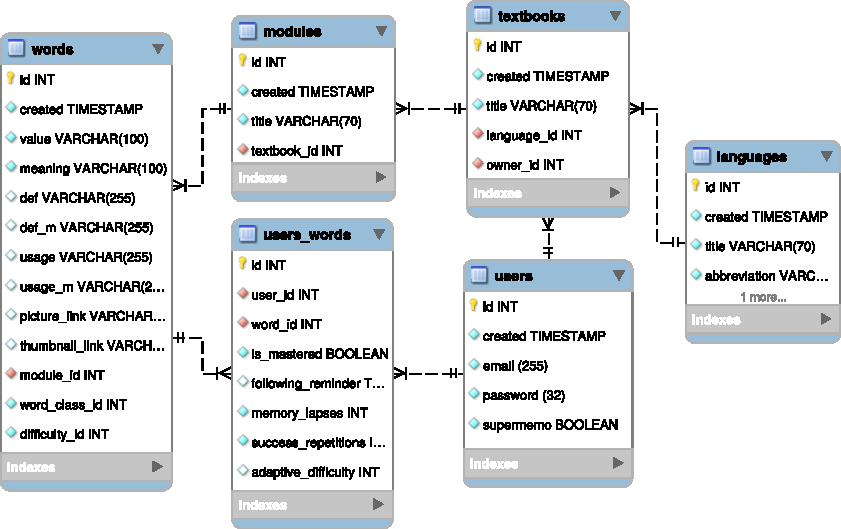
\includegraphics[scale=0.9]{../diagrams/db-model.pdf}
            \caption{Ukázka části databázového modelu zodpovědné za správu slovíček}
            \label{fig:db-model}
        \end{figure}

    \subsection{Testování}
        % \gls{api}TestCase Django REST
        % fixtures
        Testování rozhraní bylo zaměřené pouze na správnou funkčnost \gls{api}, tzn. kontrolu, zda jednotlivé dotazy vracejí správná data. Jednotkové testování krátkých logických funkcí nemělo příliš význam, jelikož v REST frameworku jde spíše o nastavení součástí a jejich spojení do jednotného celku, než o implementaci nízkoúrovňových logických bloků.
        
        Pro testování správné funkčnosti \gls{api} byla využita třída \gls{api}TestCase poskytovaná REST frameworkem. Testy jsou napsány na každou metodu každé \gls{api}. Kontrola jedné metody \gls{api} spočívala v ověření stavového kódu HTTP, dále v počtu vrácených dat, a pokud se jednalo o listy objektů, v náhodné kontrole hodnot objektu. K provádění dotazů posloužil objekt třídy \textit{\gls{api}Client}, který umožňoval jednoduše editovat hlavičky dotazu pro celou testovací sadu. 

        Užitečným nástrojem pro testování jsou tzv. \textit{fixtures}. Jsou to soubory ve formátu \gls{json}, které obsahují databázová data. Na začátku každé testovací sady je vytvořeno nové dočasné schéma v databázi, které má identickou strukturu s produkčním schématem v databázi. Dále jsou na začátku testu předány jednotlivé \textit{fixtures}, které pro účely testování naplní databázi požadovanými daty.

        \subsubsection{Závěrečné testování aplikace}
            Na závěr vývoje aplikace bylo provedeno testování uživateli, kteří nebyli součástí vývoje. Aplikace pro účely testování byla spuštěna na produkčním serveru, aby imitace reálného prostředí byla autentická. Dále byla do aplikace naimportována sada slovíček z učebnice anglického jazyka s názvem Headway Intermediate. Pro testování byli zvoleni dva dobrovolníci - žákyně základní školy, která aktuálně dochází do šesté třídy Základní školy Lesní v Liberci a dospělý člověk zabývající se podnikáním, který simuloval roli učitele v aplikaci. Během testování bylo objeveno několik drobných chyb, které byly ihned po testování opraveny. Z důvodu časového omezení nebylo otestováno externími uživateli připomínání naučených slov.

            Žákyně ihned ze začátku testování narazila na problém, že intuitivně neporozuměla konceptu testů. Aby si mohla začít procvičovat slova, musela totiž vytvořit test. Tato funkce je ale pouze spíše doplňkovou. Standardně vyučující pro žáky vytvoří testovací sady. Po vytvoření sady neměla žákyně žádný problém se spuštěním testu ani s testováním. Uživatelské rozhraní aplikace hodnotila převážně pozitivně s  drobnými výtkami na design aplikace, který pro ni byl až příliš strohý a málo barevný.

            Testování fiktivním učitelem spočívalo ve vytvoření editací a mazání učebnice, slovíček, modulů, tříd a testovacích sad. Orientace v aplikaci probíhala bez větších problémů. Nesrozumitelnou částí pro něj byla sekce pro řazení testů k jednotlivým třídám. Po drobné nápovědě se podařilo testy přiřadit k třídám.

\newpage
\section{Závěr}
    % 
    % Možné rozšíření - přidat možnost více významů slova
    % členy
    % komplexní problém - členy, více možností importu učebnic
    % další funkce například skrytí učebnice pro 
    % na základě závěrečného testování by si aplikace zasloužila vylepšit vzhled aplikace
    % tvorba nápovědy
    % návrh na zrušení definic a použití v mateřském jazyce
    V rámci této diplomové práce vznikla aplikace pro učení slovíček cizího jazyka. Jedná se o webovou službu, která umožňuje efektivně rozvíjet slovní zásobu u studentů libovolného věku. Pro zlepšení techniky učení jsou v aplikaci využity přizpůsobené algoritmy rozloženého opakování. V části zabývající se procvičování slov je využitý základ Leitnerova systému. Po procvičení slova následuje fáze připomínání slov, ve které je využit ověřený algoritmus SuperMemo. Generování slovíček v procvičování je přizpůsobováno v závislosti na úrovni uživatele, jenž je získána postupně z jeho předchozího odpovídání. 

    Aplikace umožňuje každému uživateli vytvořit vlastní učebnice se slovíčky. Slova lze importovat do aplikace v podobě formátu CSV. Ke skupinám slov v jednotlivých modulech lze v aplikaci jednoduše a rychle získat zvukovou a obrázkovou interpretaci. Z důvodu možného nevhodného obsahu obrazové formy, je uživatel nucen vybrat z navržených ten vyhovující, a tudíž proces nemůže být plně automatizován. Aplikace rovněž umožňuje vytvářet skupiny uživatelů, ve kterých lze sdílet celé učebnice.

    Aplikace umožňuje vytvářet seznamy slov. Tyto seznamy mohou být sdíleny vlastníkem skupiny mezi ostatní uživatele. Vyučující cizích jazyků tak mohou lépe žáky připravit na nadcházející lekci a zajistit tím její souvislejší průběh. 

    Do aplikace jsou také zařazeny prvky, které by mohly žáky motivovat k procvičování. Zda splňují funkci motivace, bude ověřeno až praktickým používáním. Během testování tuto funkci nebylo možné ověřit, jelikož je třeba více statistických údajů, což vyžaduje více uživatelů používajících aplikaci. Rovněž bylo složité otestovat, zda aplikace nedovolí uživateli zapomenout slovíčko, jelikož intervaly mezi jednotlivými připomenutími postupně narůstají až k týdnům a měsícům. Pochopitelně žákyně, která testování prováděla, neměla pro tak dlouhé intervaly dostatek času.

    Aplikace by si v budoucím vývoji zasloužila řadu rozšíření, zejména po designové stránce. Vzhled by bylo dobré předat profesionálnímu návrháři, který by přizpůsobil aplikaci tak, aby zaujala především mladé žáky. Aplikace by také mohla být rozšířena o další možnosti importu slovíček v podobě formátů XLS a PDF. V neposlední řadě rozšířením by mohlo být i zapracování členů přímo do struktury slovíčka, což by umožňovalo přesněji vyhodnocovat odpovědi.


\newpage
\begin{thebibliography}{99}
    
    \addcontentsline{toc}{section}{\refname}

    \bibitem{bib:terasoft}
        Terasoft a.s. \textit{Terasoft - Výukové programy} [online] 2002-10-07. [cit. 2016-12-15]. Dostupné z: \url{http://www.terasoft.cz/czpages/cd_aj15.htm}.
    
    \bibitem{bib:langsoft}
        LangSoft s.r.o. \textit{Language Teacher} [online]. [cit. 2016-12-07]. Dostupné z: \url{http://www.langsoft.cz/teacher.htm}.

    \bibitem{bib:motivace}
        KREJČOVÁ Lenka. \textit{Psychologické aspekty vzdělávání dospívajících}. 1. vyd. Praha: Grada Publishing, 2011 [cit 2016-12-18]. ISBN 978-80-247-3474-3.

    \bibitem{bib:beimiller}
        BIEMILLER Andrew, BOOTE Catherine. \textit{An effective method for building meaning vocabulary in primary grades}. Vol 98(1), Journal of Educational Psychology, 2006 [cit 2016-12-18].

    \bibitem{bib:suggestology}
        LOZANOV Georgi. \textit{Suggestology and Outlines of Suggestopedy}. 1. vyd. Gordon and Breach, 1978 [cit 2016-12-18]. ISBN 0-203-39282-5.

    \bibitem{bib:learning-vocab}
        I. S. P. Nation \textit{Learning Vocabulary in Another Language}. Cambridge University Press, 2001 [cit 2016-12-18]. ISBN 0-521-800927.

    \bibitem{bib:spaced-rep}
        Kwantlen Polytechnic University. \textit{Spaced Repetition: Remembering What You Learn} [online] 2003. [cit. 2016-12-19]. Dostupné z: \url{https://www.kpu.ca/sites/default/files/Learning%20Centres/Think_SpacedRepetition_LA.pdf}.

    \bibitem{bib:lexikologie}
        SVOBODOVÁ Jana, SVOBODOVÁ Diana, KULDANOVÁ Pavlína, GEJGUŠOVÁ Ivana, ROSOVÁ Milena, NOVÁK Radomil. \textit{Lexikologie} [online] 2003. [cit. 2016-12-19]. Dostupné z: \url{http://www.osu.cz/fpd/kcd/dokumenty/cestinapositi/lexikologie.htm}.

    \bibitem{bib:levenshtein}
         Wikimedia Foundation, Inc. \textit{Levenshtein distance} [online] 2016-12-20. [cit. 2016-12-21]. Dostupné z: \url{https://en.wikipedia.org/wiki/Levenshtein_distance}.
        
    \bibitem{bib:google-api}
        Google, Inc. \textit{Google Cloud Platform} [online]. [cit 2016-12-21]. Dostupné z: \url{https://cloud.google.com/}.

	\bibitem{bib:ebbinghaus}
		Hermann Ebbinghaus \textit{Memory: A Contribution to Experimental Psychology}. New York, 1913 [cit 25-12-2016]. ISBN 978-16-142-7166-6.

    \bibitem{bib:supermemo}
        WOZNIAK Piotr A. \textit{Repetition spacing algorithm used in SuperMemo 2002 through SuperMemo 2006} [online] 2006-04-02. [cit. 2016-12-26]. Dostupné z: \url{https://www.supermemo.com/english/algsm11.htm}.

    \bibitem{bib:spa}
        TAKADA Mikito. \textit{Single page apps in depth} [online] 2014. [cit. 2016-12-27]. Dostupné z: \url{http://singlepageappbook.com/}.

    \bibitem{bib:webpack}
        KOPPERS Tobias a spol. \textit{Webpack 2 Documentation} [online] 2016. [cit. 2016-12-26]. Dostupné z: \url{https://webpack.js.org/configuration/}.

    \bibitem{bib:babel}
        SUSCAK Marek a spol. \textit{Learn ES2015} [online] 2016. [cit. 2016-12-27]. Dostupné z: \url{https://babeljs.io/learn-es2015/}.
        
    \bibitem{bib:ecma}
        Ecma International. \textit{ECMAScript® 2015 Language Specification} [online] 2015 [cit. 2016-12-27]. Dostupné z: \url{http://www.ecma-international.org/ecma-262/6.0/index.html}.

    \bibitem{bib:jsx}
        Facebook Inc. \textit{\gls{js}X In Depth} [online] 2016 [cit. 2016-12-28]. Dostupné z: \url{https://facebook.github.io/react/docs/jsx-in-depth.html}.

    \bibitem{bib:react}
        Facebook Inc. \textit{React Components and Props} [online] 2016 [cit. 2016-12-28]. Dostupné z: \url{https://facebook.github.io/react/docs/components-and-props.html}.
        
    \bibitem{bib:mobx}
        WESTSTRATE Michel a spol. \textit{MobX Core Concepts} [online] 2016 [cit. 2016-12-28].
        Dostupné z: \url{https://mobxjs.github.io/mobx/index.html}.

    \bibitem{bib:django}
        Django Software Foundation. \textit{Django documentation} [online] 2015 [cit. 2016-12-28]. Dostupné z: \url{http://www.docs.djangoproject.com/en/}.

    \bibitem{bib:django-rest}
        CHRISTIE Tom. \textit{Django REST framework} [online] 2015 [cit. 2016-12-28]. Dostupné z: \url{http://www.django-rest-framework.org/}.

    \bibitem{bib:csrf}
       Open Web Application Security Project. \textit{Cross-Site Request Forgery} [online] 2016-11-02 [cit. 2016-12-29]. Dostupné z: \url{https://www.owasp.org/index.php/Cross-Site_Request_Forgery_%28CSRF%29}.

    \bibitem{bib:xss}
       Open Web Application Security Project. \textit{Cross-site Scripting (XSS)} [online] 2016-11-02 [cit. 2016-12-29]. Dostupné z: \url{https://www.owasp.org/index.php/XSS}.

    \bibitem{bib:jwt}
       Auth0 Inc. \textit{Introduction to \gls{json} Web Tokens} [online] 2016-11-02 [cit. 2016-12-29]. Dostupné z: \url{https://jwt.io/introduction/}.
       
\end{thebibliography}
\end{document}
